% =============================================================================
% Dissertation Report 鈥?Xihao Wang, UCL
%
% Build:
%   cd thesis
%   pdflatex dissertation_report.tex
%   pdflatex dissertation_report.tex
%
% Font: Times New Roman equivalent (newtx), 12pt body (report class).
% For exact system Times New Roman, compile with XeLaTeX and uncomment
% the fontspec block below (comment out inputenc/T1/newtx).
%
% Edit [Degree Name] and [Student ID] on the title page if required.
% =============================================================================

\documentclass[12pt,a4paper,oneside]{report}

\usepackage[utf8]{inputenc}
\usepackage[T1]{fontenc}

% Times New Roman (12pt body via document class)
\usepackage{newtxtext,newtxmath}

% ,  Optional: exact Times New Roman via XeLaTeX , 
% \usepackage{fontspec}
% \setmainfont{Times New Roman}[Ligatures=TeX]
% \usepackage{unicode-math}
% \setmathfont{TeX Gyre Termes Math}

\usepackage[margin=2.5cm]{geometry}
\usepackage{setspace}
\usepackage{graphicx}
\graphicspath{{figures/}}
\usepackage{eso-pic}
\usepackage{hyperref}
\usepackage{xurl}  % allow line breaks in long URLs and repository paths
\usepackage{natbib}
\usepackage{booktabs}
\usepackage{multirow}
\usepackage{tabularx}
\usepackage{titlesec}
\usepackage{tikz}
\usetikzlibrary{arrows.meta,calc,positioning,shapes.geometric}

% Chapter headings: "1. Introduction" (not "Chapter 1 Introduction")
\titleformat{\chapter}[hang]
  {\normalfont\huge\bfseries}
  {\thechapter.}
  {0.8em}
  {}
\titlespacing*{\chapter}{0pt}{12pt}{18pt}

% Table of contents: "1. Introduction"
\usepackage{tocloft}
\renewcommand{\cftchapaftersnum}{.}

\hypersetup{
  colorlinks=true,
  linkcolor=black,
  citecolor=black,
  urlcolor=blue,
  pdftitle={Dissertation Report: Dual-Dataset Adversarial Robustness for Medical Image Classification},
  pdfauthor={Xihao Wang},
}

\onehalfspacing
\newcommand{\train}{\mathrm{train}}
\long\def\sectionfocus#1\par{\noindent\textbf{#1}\space\ignorespaces}
\renewcommand{\abstractname}{Abstract}
\renewcommand{\bibname}{References}

\title{Robustness Evaluation of Medical Image Classification Models:\\
A Study on Brain MRI and Chest X-Ray}
\author{Xihao Wang}
\date{August 2026}

\begin{document}

% =============================================================================
% Title Page
% =============================================================================
\begin{titlepage}
  \thispagestyle{empty}
  \AddToShipoutPictureBG*{%
    \AtPageUpperLeft{%
      \raisebox{-\height}{%
        \includegraphics[width=\paperwidth]{./UCL page header.png}%
      }%
    }%
  }
  \centering
  \vspace*{5.1cm}

  {\LARGE Robustness Evaluation of Medical Image\\[0.35em]
  Classification Models\par}
  \vspace{0.45cm}
  {\Large A Study on Brain MRI and Chest X-Ray\par}

  \vspace{1.55cm}
  {\Large Xihao Wang\par}
  \vspace{0.25cm}
  {\large Student ID: 25026936\par}
  \vspace{0.45cm}
  {\large Supervisor: Jack Ruan\par}
  \vspace{0.55cm}
  {\large Faculty of Engineering Sciences\par}
  \vspace{0.18cm}
  {\large Department of Computer Science\par}

  \vspace{1.55cm}
  {\large University College London\par}
  \vspace{0.35cm}
  {\large A Project Report Presented in Partial Fulfilment of the Degree\par}
  \vspace{0.35cm}
  {\large\itshape MSc Artificial Intelligence for Biomedicine and Healthcare\par}

  \vfill
  {\large August 2026\par}
  \vspace{0.65cm}

\end{titlepage}

% =============================================================================
% Abstract Page
% =============================================================================
\pagenumbering{roman}
\setcounter{page}{1}

\chapter*{\abstractname}
\addcontentsline{toc}{chapter}{\abstractname}

Deep learning models for medical image classification achieve high accuracy on clean test data, yet remain vulnerable to adversarial perturbations that can cause clinically dangerous misclassifications. Most existing robustness studies evaluate a single dataset, a single architecture, or a single defense in isolation, leaving open the question of whether robustness rankings and attack severity generalise across medical imaging modalities and tasks.

This dissertation report presents a systematic dual-dataset study on \emph{Brain MRI} tumour detection (NO\_TUMOR vs.\ TUMOR) and \emph{Chest X-ray} pneumonia detection (NORMAL vs.\ PNEUMONIA). Five pretrained architectures, ResNet50, DenseNet121, ResNet18, MobileNetV2, and ConvNeXt-Tiny, are fine-tuned under a unified protocol and evaluated against $L_\infty$ white-box attacks (FGSM, PGD, BIM with ten steps, and DeepFool as a supplementary attack). Momentum Iterative FGSM (MIM) is evaluated on ResNet50 only to compare relative attack strength. On Brain MRI, the study further evaluates PGD adversarial training (PGD-AT) for ResNet50 and DenseNet121, and a four-condition Gaussian smoothing defence (D0--D3) combining inference-time blur with PGD-AT.

Within each task, results show that clean accuracy does not predict adversarial robustness: ConvNeXt-Tiny attains the highest clean accuracy on both datasets but collapses under iterative attacks (PGD/BIM) from $\epsilon = 2/255$ onward, whereas ResNet50 is the most robust model on Brain MRI. A cross-task comparison reveals that architecture robustness rankings are \emph{task-dependent}. For example, ResNet50 robust accuracy at $\epsilon = 4/255$ under PGD drops from 7.60\% on Brain MRI to 0.23\% on Chest X-ray, while the relative ordering of attack strength on ResNet50 (MIM and PGD strongest, FGSM weakest) is consistent across both domains. On Brain MRI, combining PGD-AT with all-input Gaussian blur (condition D3) raises PGD robust accuracy at $\epsilon = 4/255$ from 7.52\% (D0, standard model) to 96.53\%, demonstrating that training-time and inference-time defences are complementary.

These findings support the use of cross-modal robustness benchmarking before clinical deployment, and show that layered defences can substantially improve resilience on the primary Brain MRI task without requiring retraining alone.

\vspace{1.2em}
\noindent\textbf{Keywords:}
adversarial robustness,
medical image classification,
brain MRI,
chest X-ray,
PGD adversarial training,
Gaussian smoothing,
cross-task comparison,
ResNet50,
ConvNeXt-Tiny

\newpage

% =============================================================================
% Main chapters
% =============================================================================
\tableofcontents
\clearpage
\listoffigures
\clearpage
\listoftables
\newpage
\pagenumbering{arabic}
\setcounter{page}{1}

\chapter{Introduction}
\label{ch:introduction}

\section{Background and Motivation}
\label{sec:background}

\sectionfocus{High clean accuracy is insufficient for safety-critical medical imaging because small adversarial perturbations can expose severe and clinically relevant model fragility.}

Deep learning has become a central technology in medical image analysis, supporting tasks ranging from chest radiograph screening to brain tumour detection on magnetic resonance imaging (MRI). Convolutional neural networks (CNNs) and their modern variants routinely achieve high classification accuracy on held-out test sets, often matching or approaching the performance of specialist clinicians on specific benchmarks~\cite{esteva2017dermatologist,rajpurkar2017chexnet}. In pneumonia screening from chest X-rays, computer-aided systems can flag abnormal pulmonary patterns and shorten the time between image acquisition and clinical review~\cite{kermany2018identifying}. Similarly, MRI-based models can assist in distinguishing tumour-bearing scans from normal studies, offering a scalable adjunct to expert radiological interpretation~\cite{litjens2017survey}. The potential clinical benefit is substantial: earlier detection and triage may improve outcomes for conditions such as pneumonia and intracranial tumours, where delayed diagnosis is associated with increased morbidity and mortality.

Despite this promise, the deployment of medical AI in safety-critical settings raises concerns that extend beyond performance on clean, curated datasets. \citet{szegedy2014intriguing} demonstrated that deep neural networks are vulnerable to \emph{adversarial examples}: inputs formed by adding small, often imperceptible perturbations that cause the model to produce confident but incorrect predictions. Subsequent work showed that such vulnerabilities persist under realistic threat models, including bounded $L_\infty$ perturbations generated by iterative procedures such as the projected gradient descent (PGD) attack~\cite{madry2018towards}. In medical imaging, adversarial perturbations need not correspond to physically realisable acquisition artefacts; rather, they expose fragility in the decision boundaries learned by the model. This fragility could, in principle, be exploited or arise inadvertently through preprocessing pipelines, display transformations, or malicious manipulation of digital records~\cite{finlayson2019adversarial,ma2021understanding}.

The clinical stakes of misclassification are asymmetric. A false negative in pneumonia detection may delay antibiotic or supportive treatment; a false negative in tumour screening may defer definitive diagnosis. Conversely, excessive false positives increase workload and downstream imaging costs. Standard benchmark metrics computed on clean data, including accuracy, sensitivity, and area under the receiver operating characteristic curve, therefore provide an incomplete picture of reliability. A model that achieves 98\% clean accuracy may collapse to near-zero robust accuracy under PGD or basic iterative methods (BIM) at perturbation budgets as small as $\epsilon = 4/255$ in pixel space~\cite{madry2018towards,kurakin2017adversarial}. For regulators, hospital information-technology teams, and researchers, it is insufficient to report only clean performance; adversarial robustness must be characterised alongside conventional metrics~\cite{finlayson2019adversarial}.

Most robustness studies in computer vision focus on natural-image datasets such as CIFAR-10 or ImageNet~\cite{madry2018towards,dong2018mim}. Medical imaging presents distinct challenges: different texture statistics, class imbalance, smaller effective sample sizes, and modality-specific acquisition physics. A model that appears robust on one task may not generalise to another; likewise, an architecture that maximises clean accuracy on chest radiographs may not retain favourable robustness rankings on brain MRI. Existing medical AI robustness evaluations often examine a single modality, a single architecture (frequently ResNet-based transfer learning~\cite{he2016deep}), or a single defence in isolation~\cite{ma2021understanding,finlayson2019adversarial}. Cross-task comparisons under a unified experimental protocol remain relatively scarce, limiting our understanding of whether robustness rankings and attack severity transfer across clinical domains.

This dissertation report addresses that gap by conducting a systematic dual-dataset study spanning brain tumour MRI classification and paediatric chest X-ray pneumonia detection, using five representative architectures and a common suite of white-box attacks, with extended defence experiments on the brain MRI task.

\section{Research Questions}
\label{sec:problem}

\sectionfocus{The study isolates how architecture, task and dataset, attack choice, and defence design shape adversarial robustness.}

The project is guided by four research questions:
\begin{description}
  \item[\textbf{RQ1.}] \textbf{How does model architecture influence adversarial robustness in medical image classification?}

  Models with similar clean accuracy may learn different features and decision boundaries, and may therefore respond differently to the same perturbation. This question examines whether architecture choice affects robustness independently of standard predictive performance. In this dissertation, five ImageNet-pretrained architectures, ResNet50, DenseNet121, ResNet18, MobileNetV2, and ConvNeXt-Tiny, are fine-tuned under a common protocol and evaluated using matched white-box attacks. Their clean and adversarial results are compared to determine whether the clean-performance ranking is a useful guide to robust model selection.

  \item[\textbf{RQ2.}] \textbf{To what extent does adversarial robustness vary across medical image classification tasks and datasets?}

  Medical datasets differ in image formation, texture, class balance, and diagnostic target, so robustness measured in one domain may not describe behaviour in another. This question tests whether vulnerability is dependent on the classification setting rather than being an intrinsic and fixed property of an architecture. The dissertation addresses it through matched experiments on binary brain MRI tumour classification and paediatric chest X-ray pneumonia classification. The same model families, image resolution, preprocessing principles, perturbation budgets, and primary attack implementations are used so that cross-task differences can be interpreted consistently.

  \item[\textbf{RQ3.}] \textbf{How stable is the relative effectiveness of different adversarial attacks across classification tasks?}

  Robustness conclusions can depend strongly on the selected attack: a model that survives a single-step perturbation may still fail under an iterative or momentum-based method. This question considers whether the relative effectiveness of attack algorithms remains broadly consistent when the medical classification task changes. In the main experiments, FGSM, PGD, and BIM are evaluated across the five architectures. A focused ResNet50 comparison additionally includes MIM at common $L_\infty$ budgets, while DeepFool and C\&W are retained as supplementary attacks because their optimisation objectives differ from the primary fixed-budget comparison.

  \item[\textbf{RQ4.}] \textbf{To what extent can training-time and inference-time defence strategies improve the adversarial robustness of medical image classifiers?}

  Defences can modify the learned decision boundary during training or transform inputs before prediction, and the two approaches may provide complementary protection. This question investigates both the magnitude of the robustness gain and whether combining mechanisms is more effective than applying either mechanism alone. Within the scope of this dissertation, PGD adversarial training is evaluated on ResNet50 and DenseNet121, while Gaussian smoothing is tested on ResNet50 under four conditions (D0--D3). These defence experiments are conducted on brain MRI and compare standard training, inference-time smoothing, and their combination across multiple perturbation budgets.
\end{description}

Together, the four questions distinguish architecture effects, task and dataset effects, attack selection, and defence design. They remain sufficiently general to motivate the study, while the experimental choices above define the evidence used to answer them in Chapter~\ref{ch:conclusion}.

\section{Objectives and Contributions}

\sectionfocus{The project contributes a controlled dual-dataset benchmark and a focused evaluation of both training-time and inference-time protection.}

To answer the questions, five ImageNet-pretrained models, ResNet50, DenseNet121, ResNet18, MobileNetV2, and ConvNeXt-Tiny, are fine-tuned on binary brain MRI and paediatric chest X-ray tasks. FGSM, PGD, and BIM form the common five-model benchmark, while MIM is used for a focused ResNet50 attack-strength comparison. The evaluation reports clean and robust accuracy, attack success rate, sensitivity, F1, and AUC where available. The defence experiments compare standard and PGD-adversarially trained ResNet50 and DenseNet121 models, followed by a four-condition Gaussian smoothing study on ResNet50.

The resulting contribution is empirical rather than theoretical: a controlled cross-task benchmark, an explicit test of whether robustness rankings transfer between modalities, and a factorial comparison of training-time and inference-time protection. All numerical claims in the discussion are tied to held-out test results reported in Chapter~\ref{ch:results}.

\section{Scope and Organisation}
\label{sec:scope}

\sectionfocus{The empirical claims are bounded by a white-box threat model, matched $L_\infty$ attacks, and defence experiments concentrated on brain MRI.}

The threat model is \emph{white-box}: attackers are assumed to know model parameters and gradients, yielding conservative robustness estimates relative to black-box transfer attacks~\cite{papernot2017practical}. MIM is applied only to ResNet50 for attack-strength comparison rather than a five-model leaderboard. PGD adversarial training and Gaussian smoothing are restricted to brain MRI (Gaussian conditions on ResNet50), while chest X-ray experiments stop at standard-model attack evaluation. DeepFool coverage is partial across architectures owing to computational cost; FGSM, PGD, and BIM constitute the primary comparison trio. Within these boundaries, the work provides a coherent, reproducible evidence base anchored in publicly available datasets and documented training scripts.

Chapter~\ref{ch:related} reviews the relevant attacks, defences, and medical-imaging evidence. Chapter~\ref{ch:methods} describes the data, training, threat model, and evaluation protocol. Results are presented in Chapter~\ref{ch:results} and interpreted in Chapter~\ref{ch:discussion}; the final two chapters state the conclusions and prioritise the work that remains.

Figure~\ref{fig:experimental-workflow} summarises the experimental pipeline. Both datasets pass through the same preprocessing and standard-training stages before clean and adversarial evaluation. The pipeline then separates into a cross-task robustness analysis and a brain-MRI defence study, after which all outcomes are assessed using a common set of metrics.

\begin{figure}[htbp]
  \centering
  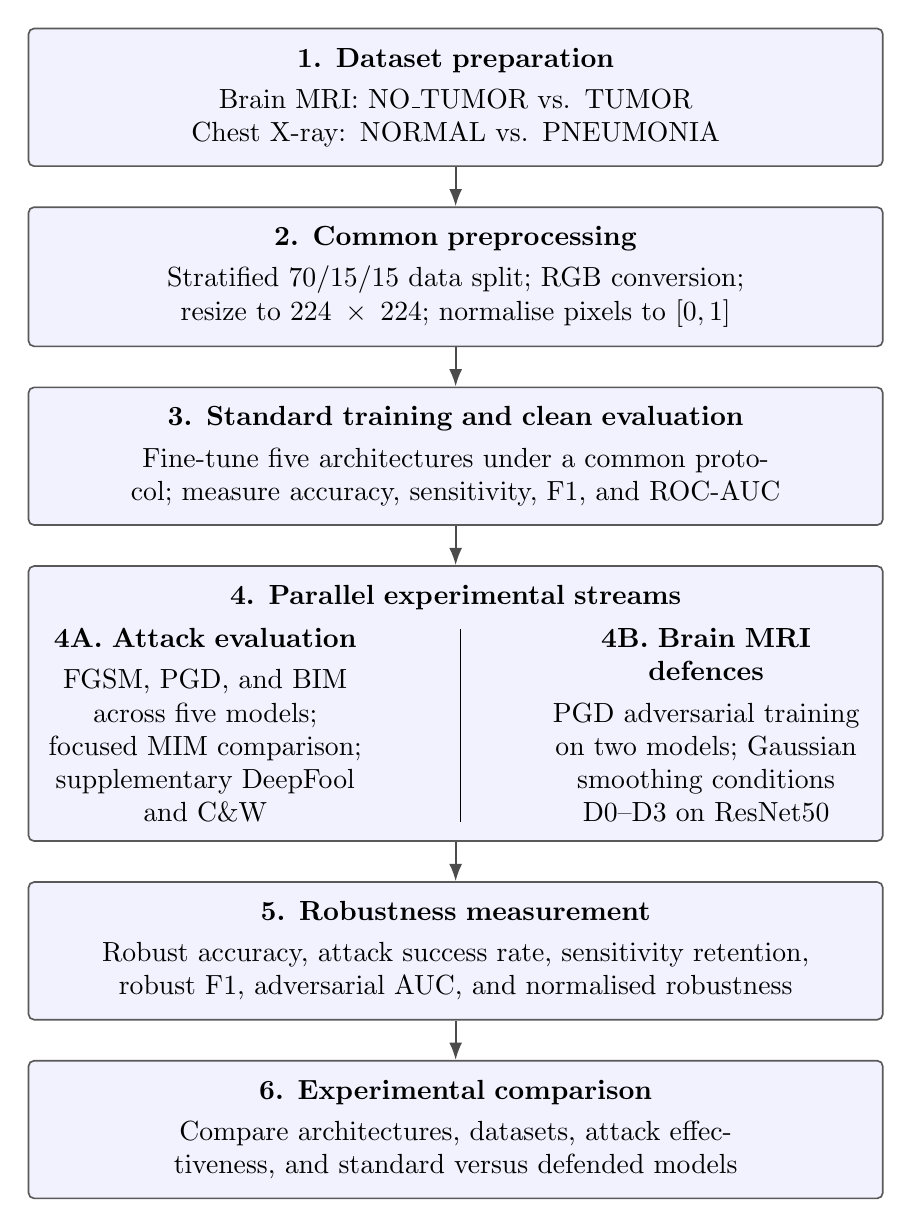
\begin{tikzpicture}[
    node distance=5mm,
    every node/.style={font=\normalsize, align=center},
    stage/.style={
      rectangle, rounded corners=2pt, draw=black!65, line width=0.6pt,
      fill=blue!5, text width=0.86\textwidth, minimum height=11mm,
      inner xsep=6pt, inner ysep=7pt
    },
    flow/.style={-{Latex[length=2.2mm]}, line width=0.7pt, draw=black!70}
  ]
    \node[stage] (data) {\textbf{1. Dataset preparation}\\[1mm]
      Brain MRI: NO\_TUMOR vs. TUMOR \qquad Chest X-ray: NORMAL vs. PNEUMONIA};
    \node[stage, below=of data] (preprocess) {\textbf{2. Common preprocessing}\\[1mm]
      Stratified 70/15/15 data split; RGB conversion; resize to $224\times224$; normalise pixels to $[0,1]$};
    \node[stage, below=of preprocess] (train) {\textbf{3. Standard training and clean evaluation}\\[1mm]
      Fine-tune five architectures under a common protocol; measure accuracy, sensitivity, F1, and ROC-AUC};
    \node[stage, below=of train] (experiments) {\textbf{4. Parallel experimental streams}\\[2mm]
      \begin{minipage}{0.39\textwidth}
        \centering
        \textbf{4A. Attack evaluation}\\[1mm]
        FGSM, PGD, and BIM across five models; focused MIM comparison; supplementary DeepFool and C\&W
      \end{minipage}
      \hfill\vrule\hfill
      \begin{minipage}{0.39\textwidth}
        \centering
        \textbf{4B. Brain MRI defences}\\[1mm]
        PGD adversarial training on two models; Gaussian smoothing conditions D0--D3 on ResNet50
      \end{minipage}};
    \node[stage, below=of experiments] (metrics) {\textbf{5. Robustness measurement}\\[1mm]
      Robust accuracy, attack success rate, sensitivity retention, robust F1, adversarial AUC, and normalised robustness};
    \node[stage, below=of metrics] (compare) {\textbf{6. Experimental comparison}\\[1mm]
      Compare architectures, datasets, attack effectiveness, and standard versus defended models};

    \draw[flow] (data) -- (preprocess);
    \draw[flow] (preprocess) -- (train);
    \draw[flow] (train) -- (experiments);
    \draw[flow] (experiments) -- (metrics);
    \draw[flow] (metrics) -- (compare);
  \end{tikzpicture}
  \caption{Experimental workflow used for clean classification, adversarial robustness evaluation, cross-task comparison, and defence assessment.}
  \label{fig:experimental-workflow}
\end{figure}

\chapter{Related Work}
\label{ch:related}

\sectionfocus{Prior research establishes the vulnerability of medical image classifiers but leaves cross-task robustness and combined defence behaviour insufficiently characterised.}

This chapter first reviews the growth and clinical importance of medical image classification as a broad field, and then examines adversarial attacks, defences, evidence from robustness studies, and the remaining research gaps.

\section{Growth and Importance of Medical Image Classification}

\sectionfocus{Medical image classification has become an important area of clinical artificial intelligence because it can convert increasingly large imaging archives into reproducible evidence for detection, triage, and diagnostic support.}

The adoption of deep learning in medical imaging extends well beyond any single modality or disease. The survey by \citet{litjens2017survey} documents applications across radiography, computed tomography, magnetic resonance imaging, ultrasound, retinal imaging, dermatology, and histopathology. Depending on the clinical question, classification models may distinguish normal from abnormal studies, identify a disease category, estimate severity, or prioritise examinations for specialist review. This breadth has made image classification one of the most visible uses of machine learning in healthcare.

\paragraph{Expanding clinical applications.}
Evidence of this growth can be seen across several specialties. \citet{esteva2017dermatologist} demonstrated deep neural network classification of skin lesions at dermatologist-comparable performance on a constrained benchmark. In radiology, \citet{rajpurkar2017chexnet} applied DenseNet121 to pneumonia detection from chest radiographs, while \citet{kermany2018identifying} showed that transfer-learned models could support classification across retinal and paediatric chest imaging tasks. Related work surveyed by \citet{litjens2017survey} includes tumour classification, lesion characterisation, tissue categorisation, and other diagnostic decisions across two- and three-dimensional imaging. Collectively, these studies show that medical image classification is not a narrow application tied to one dataset, but a broad methodological approach used across organs, diseases, and acquisition technologies.

\paragraph{Clinical and operational importance.}
The importance of classification models arises partly from the growing volume and complexity of medical imaging. Automated predictions can provide a second opinion, flag potentially urgent examinations, support screening programmes, and reduce repetitive review in high-volume workflows. They may also improve consistency where access to specialist expertise is limited. However, these systems are intended to influence safety-critical decisions, and the costs of false negatives and false positives are not symmetric. High benchmark accuracy is therefore necessary but insufficient: clinically relevant evaluation must also consider sensitivity, specificity, calibration, dataset shift, and failure under unexpected or deliberately manipulated inputs.

\paragraph{Transfer learning and the robustness problem.}
Medical imaging datasets are often smaller and more expensive to annotate than natural-image collections. ImageNet pretraining followed by domain-specific fine-tuning has consequently become a common strategy~\cite{deng2009imagenet,he2016deep}. Transfer learning can reduce data requirements and improve clean performance by reusing general visual features, but it does not guarantee that the resulting decision boundary is stable. \citet{tsipras2019robustness} argue that features favoured by standard accuracy may differ from those required for adversarial robustness. As medical classifiers become more widely studied and deployed, robustness evaluation therefore becomes part of assessing whether apparent predictive success represents dependable behaviour.

\section{Robustness Research in Medical Image Classification}
\label{sec:rw-medical-robust}

\sectionfocus{Existing studies consistently show that medical image classifiers can fail under small perturbations, but the measured level of robustness changes with modality, architecture, attack, dataset, and evaluation metric.}

Early work used adversarial examples as a stress test for medical models rather than treating clean test accuracy as sufficient evidence of generalisation. \citet{paschali2018generalizability} compared skin-lesion classification and whole-brain segmentation models and found that networks with comparable clean performance could differ substantially in robustness. \citet{finlayson2019adversarial} subsequently demonstrated attack vulnerability in fundus imaging, dermatology, and chest radiography, drawing attention to the safety and incentive risks of manipulating medical predictions.

Later studies broadened the range of datasets and questions. \citet{hirano2021universal} evaluated targeted and untargeted universal perturbations across skin, OCT, and chest X-ray classification with six architectures, showing that one image-agnostic perturbation could affect many inputs. \citet{rodriguez2022complexity} studied model complexity on chest X-ray, dermoscopy, and OCT data and reported that smaller standard models could be more robust than larger networks with similar clean accuracy. \citet{ghamizi2023evaluating} showed that chest X-ray robustness conclusions vary with the dataset, architecture, metric, label structure, and clinical threat model. Together with the survey and empirical analysis of \citet{ma2021understanding}, these findings establish robustness as an evaluation problem in its own right rather than a direct consequence of clean performance.

Table~\ref{tab:medical-robustness-literature} compares representative studies. The final column is important because the studies answer related but not identical questions; their results should not be pooled as though they used one common benchmark.

\begin{table}[htbp]
  \centering
  \caption{Representative research on adversarial robustness in medical image classification.}
  \label{tab:medical-robustness-literature}
  \small
  \begin{tabularx}{\textwidth}{p{2.55cm} p{3.55cm} X}
    \toprule
    Study & Medical scope & Contribution and limitation \\
    \midrule
    Paschali et al. (2018) & Skin-lesion classification; brain segmentation & Used adversarial examples to separate clean generalisation from robustness; mixed classification and segmentation rather than a matched cross-task classification benchmark. \\
    Finlayson et al. (2019) & Fundus, dermatology, and chest radiography & Demonstrated clinically relevant white- and black-box vulnerability across modalities; focused on attack feasibility rather than architecture ranking. \\
    Hirano et al. (2021) & Skin, retinal OCT, and chest X-ray classification & Compared six architectures under targeted and untargeted universal perturbations and tested adversarial retraining; centred on UAPs rather than per-image PGD/BIM attacks. \\
    Ma et al. (2021) & Multiple medical analysis tasks & Analysed medical attack surfaces and detection behaviour across applications; broad in scope but not a unified dual-dataset model benchmark. \\
    Rodriguez et al. (2022) & Chest X-ray, dermoscopy, and OCT classification & Linked lower model complexity to greater robustness among standard models with similar clean accuracy; used a specialised complexity-controlled model family. \\
    Ghamizi et al. (2023) & Three chest X-ray datasets, seven models, 18 findings & Showed that dataset, metric, labels, and threat model can change robustness conclusions; restricted to chest radiography. \\
    \bottomrule
  \end{tabularx}
\end{table}

The literature therefore supports three conclusions relevant to this dissertation. First, clean accuracy cannot substitute for adversarial evaluation. Second, robustness is conditional on the task and protocol, so apparently conflicting results may reflect different threat models rather than experimental error. Third, systematic cross-task comparisons remain limited: broad multi-modality studies often use different tasks or attacks in each domain, whereas tightly controlled studies commonly remain within one modality.

\section{Research on Adversarial Attacks and Defences}
\label{sec:rw-attacks}

\sectionfocus{Attack research has progressed from simple gradient perturbations to iterative, momentum, optimisation, universal, and adaptive methods, while defence research spans robust training, detection, preprocessing, feature denoising, and certification.}

\paragraph{Gradient-based and optimisation attacks.}
FGSM uses one signed-gradient update and provides a fast first-order baseline~\cite{goodfellow2015explaining}. BIM repeats smaller signed-gradient steps~\cite{kurakin2017adversarial}, while PGD adds projection and typically a random start, making it a standard empirical test of $L_\infty$ robustness~\cite{madry2018towards}. MIM accumulates momentum to stabilise update directions and improve attack effectiveness and transferability~\cite{dong2018mim}. DeepFool estimates a nearby decision boundary to obtain a small-norm perturbation~\cite{moosavi2016deepfool}, whereas Carlini--Wagner attacks optimise a margin-based objective and were developed to overcome earlier defensive mechanisms~\cite{carlini2017towards}. These methods test different properties, so robust accuracy under one attack should not be interpreted as a universal robustness score.

\paragraph{Medical and alternative attack settings.}
Medical studies have adapted these attacks to dermoscopy, retinal imaging, radiography, and other diagnostic tasks. \citet{finlayson2019adversarial} considered both white-box manipulation and more constrained attack settings. \citet{hirano2021universal} studied universal perturbations that are shared across images, which differ from the per-image perturbations generated by FGSM or PGD. Work surveyed by \citet{dong2023survey} also includes transfer-based black-box attacks, physically or acquisition-motivated perturbations, and backdoor or poisoning scenarios. This variety matters clinically because an attacker with model gradients, a malicious data provider, and an uncontrolled acquisition pipeline represent different threat assumptions.

\paragraph{Training-time defences.}
Adversarial training incorporates attacked samples into optimisation and remains one of the most reliable empirical defences. The PGD min--max formulation of \citet{madry2018towards} explicitly optimises worst-case loss within a perturbation set. Ensemble adversarial training exposes a model to examples transferred from multiple sources~\cite{tramer2018ensemble}. In medical imaging, \citet{hirano2021universal} evaluated adversarial retraining against universal perturbations, while \citet{li2020defending} proposed semi-supervised adversarial training to address limited medical labels. These approaches can improve robustness but increase training cost and may reduce clean accuracy or specialise to the training threat model.

\paragraph{Inference-time, detection, and certified defences.}
Input transformations attempt to remove perturbation components before classification; examples include smoothing, compression, reconstruction, and frequency-domain processing. Feature denoising instead modifies internal representations~\cite{xie2019feature}. Adversarial detection seeks to reject suspicious inputs: \citet{li2020defending}, for example, combined semi-supervised training with unsupervised adversarial detection on OCT data. Randomised smoothing aggregates predictions from noisy copies and can provide certified $L_2$ guarantees~\cite{cohen2019certified}, although its computational and statistical requirements differ from deterministic Gaussian filtering. The review by \citet{dong2023survey} concludes that medical defences remain difficult to compare fairly because studies vary in attack adaptivity, modality, perturbation norm, and reporting practice.

Overall, the attack--defence literature resembles an arms race: a defence that appears effective under a weak or non-adaptive attack may fail when the attacker accounts for it. Consequently, this dissertation uses multiple attacks, reports the threat model explicitly, and treats Gaussian smoothing as an empirical preprocessing defence rather than a certified guarantee. Section~\ref{sec:rw-gaps} identifies the remaining gaps addressed by the experimental design.

\section{Research Gaps}
\label{sec:rw-gaps}

\sectionfocus{The central gap is the absence of a unified cross-task comparison that separates architectural robustness, attack effectiveness, and layered defence gains.}

\textbf{Existing medical robustness benchmarks are commonly limited to a single imaging modality and a small number of architectures.} This makes it difficult to determine whether an observed result reflects a general property of a model family or a peculiarity of one dataset. The present dissertation responds to this limitation by evaluating brain MRI tumour classification and chest X-ray pneumonia classification under a harmonised experimental protocol. Five architectures, ResNet50, DenseNet121, ResNet18, MobileNetV2, and ConvNeXt-Tiny, are included to represent residual, densely connected, lightweight, and modern convolutional designs rather than relying on one reference network alone.

\textbf{Attack coverage and cross-task comparison also remain inconsistent across prior studies.} Medical robustness work often reports FGSM, PGD, or a small subset of available attacks, while the datasets, perturbation budgets, and evaluation metrics vary between experiments. Consequently, attack results from different publications cannot always be compared directly. This dissertation applies FGSM, PGD, and BIM across the principal model benchmark and supplements the ResNet50 analysis with MIM, DeepFool, and Carlini--Wagner attacks. Using matched $\epsilon$ values on brain MRI and chest X-ray makes it possible to examine whether architectural robustness and the relative effectiveness of attacks remain stable when the classification task changes.

\textbf{Defence mechanisms are frequently assessed separately rather than as complementary components of a robustness strategy.} Prior studies may evaluate adversarial training or an inference-time transformation, but fewer experiments compare their independent and combined effects within the same setting. The brain MRI experiments therefore contrast a standard model, PGD adversarial training, Gaussian input smoothing, and a combination of training-time and inference-time protection. The D0--D3 conditions provide a controlled way to distinguish the contribution of each component, although the defence study is deliberately restricted to brain MRI and is not presented as evidence of universal clinical protection.

\textbf{Finally, inconsistent metrics and incomplete reporting reduce reproducibility.} Normalised robustness and sensitivity under attack have been advocated for fairer medical evaluation~\cite{ma2021understanding}, but they are not reported consistently alongside clean accuracy and attack success rate. This dissertation brings these measures together in a documented dual-dataset benchmark. In summary, its contribution is not simply the use of more models or attacks, but a unified design that separates the effects of architecture, classification task, attack method, and defence configuration. Section~3 describes how this design is implemented, and Section~4 reports the resulting evidence.

\chapter{Materials and Methods}
\label{ch:methods}

\sectionfocus{The methodology uses matched data processing, training, attacks, and metrics to make architecture- and task-level robustness comparisons as controlled as possible.}

This section describes the datasets, models, training procedures, attack and defence protocols, evaluation metrics, and cross-task comparison methodology used in the experiments reported in Section~4. Experiments proceed in a fixed order: standard training of five CNN architectures on each dataset, within-task adversarial evaluation using FGSM, PGD, BIM, and supplementary DeepFool, ResNet50 attack-strength comparison including MIM on both datasets, cross-task alignment of robustness and attack-strength tables at matched $\epsilon$ values, and brain MRI defences comprising PGD-AT for ResNet50 and DenseNet121 followed by Gaussian smoothing conditions D0--D3 on ResNet50. All attacks share hyperparameters across tasks unless noted. Chest X-ray serves as an attack-only validation domain; PGD-AT and Gaussian experiments are not repeated on chest X-ray to preserve depth on the primary brain MRI task while still enabling cross-task robustness comparison of standard models.

\section{Datasets and Preprocessing}
\label{sec:methods-data}

\sectionfocus{Both classification tasks use harmonised splits, input resolution, colour representation, and normalisation to support a controlled cross-task comparison.}

The brain MRI dataset is sourced from the Hugging Face repository \url{usamaJabar/brain-tumor-mri-classification-merged}. Original multi-class labels (glioma, meningioma, pituitary, no\_tumor) are mapped to a binary problem: NO\_TUMOR (label~0) versus TUMOR (label~1), where all tumour subtypes are merged into the positive class. All on-disk splits are merged and re-partitioned with stratified sampling and random seed~42 into 70\% training, 15\% validation, and 15\% test, yielding a test set of approximately 1{,}356 images used for all reported metrics. The chest X-ray dataset follows the paediatric pneumonia collection described by \citet{kermany2018identifying}, with class folders \texttt{NORMAL} (label~0) and \texttt{PNEUMONIA} (label~1); original \texttt{train} and \texttt{test} directories are concatenated and split stratified into 70\% train, 15\% validation, and 15\% test (seed~42), mirroring the brain MRI protocol. Both tasks load images as RGB tensors at $224 \times 224$ pixels, rescale to $[0,1]$ by dividing pixel values by~255, and use binary sigmoid outputs with the same batch size during training and attack evaluation. Using identical spatial resolution, colour mode, and normalisation across tasks ensures that cross-task differences in robustness are attributable to modality and decision-boundary effects rather than preprocessing mismatch. Table~\ref{tab:dataset-summary} summarises the two datasets.

\begin{table}[htbp]
  \centering
  \caption{Dataset summary and preprocessing.}
  \label{tab:dataset-summary}
  \small
  \begin{tabular}{p{2.2cm}p{4.8cm}p{4.8cm}}
    \toprule
    Property & Brain MRI & Chest X-ray \\
    \midrule
    Source & Hugging Face merged MRI & Kermany et al.\ paediatric CXR \\
    Classes & NO\_TUMOR / TUMOR & NORMAL / PNEUMONIA \\
    Label merge & Multi-class tumour $\rightarrow$ TUMOR & Native binary \\
    Split & 70 / 15 / 15 (stratified, resplit) & 70 / 15 / 15 (stratified, resplit) \\
    Input & $224 \times 224$ RGB, scale $1/255$ & $224 \times 224$ RGB, scale $1/255$ \\
    Test set & $1{,}356$ images & $876$ images \\
    \bottomrule
  \end{tabular}
\end{table}

Figure~\ref{fig:dataset-samples} shows representative examples from each class after resizing to the $224 \times 224$ RGB input used in all experiments. Brain MRI panels illustrate the binary mapping: a \texttt{no\_tumor} slice (negative class) and a glioma case merged into \texttt{TUMOR} (positive class). Chest X-ray panels show a \texttt{NORMAL} paediatric frontal radiograph and a \texttt{PNEUMONIA} case with visible consolidation; both modalities are replicated to three channels before normalisation to $[0,1]$.

\begin{figure}[htbp]
  \centering
  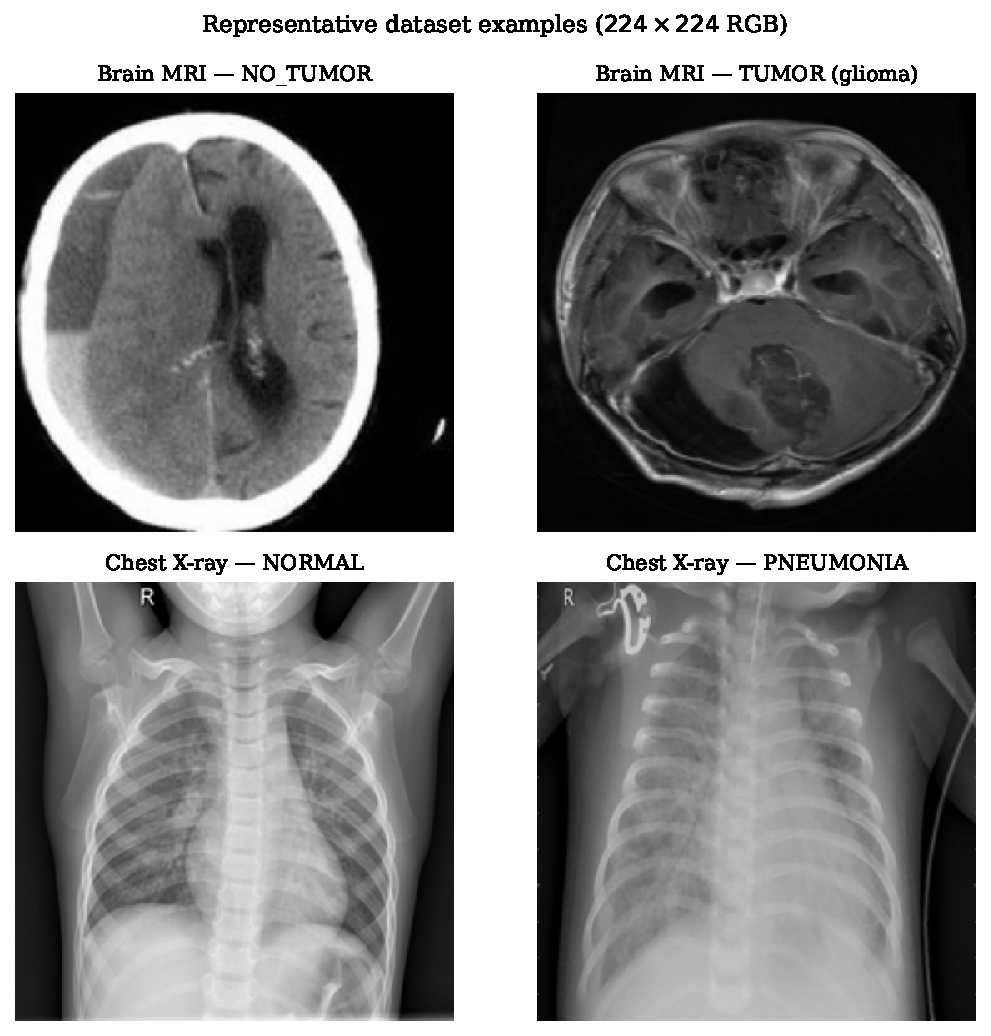
\includegraphics[width=0.92\textwidth]{figures/dataset_samples.pdf}
  \caption{Representative examples from the brain MRI and chest X-ray datasets. Top row: \texttt{NO\_TUMOR} (left) and \texttt{TUMOR} represented by glioma (right). Bottom row: \texttt{NORMAL} (left) and \texttt{PNEUMONIA} (right) chest radiographs. All panels are resized to $224 \times 224$ pixels in RGB, matching the preprocessing pipeline described above.}
  \label{fig:dataset-samples}
\end{figure}

After resplitting, the brain MRI corpus comprises approximately 9{,}040 images in total, with the positive TUMOR class forming a modest majority (roughly 60--65\% of samples after merging glioma, meningioma, and pituitary labels). The chest X-ray corpus comprises 5{,}856 frontal radiographs in total, with PNEUMONIA accounting for approximately 72.9\% of merged samples, a stronger imbalance than on brain MRI. Stratified splitting preserves these class proportions in train, validation, and test partitions. No intensity normalisation beyond scaling to $[0,1]$ is applied: both datasets are treated as three-channel RGB inputs to match ImageNet-pretrained backbones, with single-channel source images replicated across channels. This choice follows common transfer-learning practice but implies that modality-specific preprocessing (histogram equalisation, lung-field cropping, skull-stripping) was not explored; any robustness gain from such steps remains outside the present protocol. Both datasets are publicly available research corpora without patient-identifiable metadata in the released file structure; no additional ethical approval was required beyond the terms of use of the source repositories, though clinical deployment would require separate governance review.

\section{Model Architectures and Training}
\label{sec:methods-training}

\sectionfocus{Five representative transfer-learning architectures are trained under a common optimisation protocol so that robustness differences are not confounded by incompatible training settings.}

Five ImageNet-pretrained architectures are fine-tuned: ResNet50 and ResNet18~\cite{he2016deep}, DenseNet121~\cite{huang2017densely}, MobileNetV2~\cite{sandler2018mobilenetv2}, and ConvNeXt-Tiny~\cite{liu2022convnet}. Each model replaces the ImageNet classification head with global average pooling followed by a single sigmoid unit for binary cross-entropy training. ConvNeXt-Tiny uses a GPU compatibility patch for depthwise convolution under DirectML; weights are loaded from task-specific checkpoints after fine-tuning. The five architectures span a deliberate capacity--efficiency spectrum: ResNet50 ($\approx$25.6M parameters) is the de facto medical imaging baseline and the reference model for attack-strength and Gaussian studies; DenseNet121 ($\approx$8.0M) represents dense feature reuse with strong radiograph performance in prior work~\cite{rajpurkar2017chexnet}; ResNet18 ($\approx$11.7M) tests whether a shallower residual network trades clean accuracy for boundary stability; MobileNetV2 ($\approx$3.5M) approximates edge-deployable latency constraints; and ConvNeXt-Tiny ($\approx$28.3M) represents a modern ConvNet design with aggressive data-augmentation-style training defaults that achieve the highest clean scores in Section~4. Holding the training recipe constant across this set isolates architectural effects from optimisation noise as far as practicable.

Training follows a two-phase transfer-learning schedule common to both tasks. In phase one, ImageNet convolutional layers are frozen and only the new head is trained for five epochs with SGD (learning rate~0.02, momentum~0.9, decay~0.01). In phase two, all layers are unfrozen and training continues with reduced learning rate (0.01 for ResNet50; architecture-specific rates for other models) and early stopping on validation loss. Batch size~32, random seed~42, class-weighted loss to mitigate imbalance, and RGB input at $224 \times 224$ are held constant where possible. For brain MRI, validation accuracy is capped during fine-tuning to avoid degenerate solutions at 100\% validation accuracy that can destabilise adversarial evaluation. Table~\ref{tab:train-hyper} lists the principal training settings.

\begin{table}[htbp]
  \centering
  \caption{Standard model training hyperparameters (both tasks).}
  \label{tab:train-hyper}
  \begin{tabular}{ll}
    \toprule
    Hyperparameter & Value \\
    \midrule
    Optimiser & SGD (momentum 0.9) \\
    Batch size & 32 \\
    Input shape & $224 \times 224 \times 3$ \\
    Phase 1 epochs & 5 (frozen backbone) \\
    Phase 2 epochs & Up to 30 (early stopping) \\
    Loss & Binary cross-entropy with class weights \\
    Output activation & Sigmoid (threshold 0.5 at inference) \\
    Random seed & 42 \\
    \bottomrule
  \end{tabular}
\end{table}

\section{Adversarial Attack and Defence Protocol}
\label{sec:methods-attacks}

\sectionfocus{Matched perturbation budgets and attack settings establish the main robustness benchmark, while PGD adversarial training and Gaussian smoothing define the defence study.}

All primary attacks operate in a white-box setting: the attacker knows model parameters and gradients. Perturbations are bounded in $L_\infty$ norm by~$\epsilon$, with
\[
  \|\delta\|_\infty \le \epsilon, \quad x_{\mathrm{adv}} = \mathrm{clip}(x + \delta,\, 0,\, 1).
\]
Pixel values lie in $[0,1]$ after rescaling. The attack budget set is $\epsilon \in \{1,2,3,4,5,6,8\}/255$; cross-task summaries emphasise $\epsilon = 2/255$ and $4/255$. FGSM~\cite{goodfellow2015explaining} applies one signed-gradient step of magnitude~$\epsilon$. PGD~\cite{madry2018towards} uses ten iterations with step size $\alpha = \epsilon / 10$, uniform random start within the $\epsilon$-ball, and projection after each step. BIM~\cite{kurakin2017adversarial} uses the same $\alpha$ and ten iterations but without random start (deterministic init at clean~$x$). MIM~\cite{dong2018mim} adds momentum ($\mu = 1.0$) over ten iterations and is evaluated on ResNet50 only for attack-strength ranking. DeepFool~\cite{moosavi2016deepfool} approximates minimal perturbations; results are binned by $\epsilon$ for comparison with partial coverage on some architectures owing to compute cost. C\&W~\cite{carlini2017towards} is implemented as an $L_\infty$-bounded logit-margin attack (ten steps, $\kappa = 0$, $\alpha = \epsilon/10$) on ResNet50 only, reported separately from the primary attack-strength table because its optimisation objective differs from loss-maximisation PGD/BIM. Attacks are generated on the held-out test set; when robust accuracy reaches 0\% at a given~$\epsilon$, higher budgets are not re-run if monotonicity implies the result remains zero (documented for ConvNeXt-Tiny PGD on chest X-ray).

Defence experiments are conducted on brain MRI only. PGD-AT~\cite{madry2018towards} is applied to ResNet50 and DenseNet121, initialised from their standard fine-tuned checkpoints rather than from ImageNet weights alone, so that adversarial fine-tuning begins from task-adapted representations. During each training minibatch, half of the examples are replaced by PGD adversarial counterparts generated on the fly with $\epsilon_{\mathrm{train}} = 4/255$, step size $\alpha = \epsilon/10$, and ten inner PGD steps with random start within the $L_\infty$ ball; the loss on the mixed batch is binary cross-entropy averaged over clean and adversarial inputs (mix ratio~0.5). All convolutional layers remain trainable throughout PGD-AT; optimisation uses SGD with the same momentum and weight decay as standard fine-tuning, run for ten epochs without early stopping so that robustness gains are comparable across ResNet50 and DenseNet121. Checkpoints with the best validation robust accuracy under a lightweight PGD probe are retained for test evaluation. This procedure follows the Madry \emph{et al.}\ min--max formulation at a single training budget matched to the primary evaluation budget ($\epsilon = 4/255$), rather than scheduling $\epsilon$ over training. A deterministic Gaussian blur (PIL \texttt{GaussianBlur}, radius~$\sigma = 1.0$) is applied at inference time in four conditions on ResNet50 (Table~\ref{tab:d0-d3}). Attacks for the Gaussian study are restricted to PGD and BIM at $\epsilon \in \{2/255, 4/255\}$ with ten steps, matching the primary robustness tables.

\begin{table}[htbp]
  \centering
  \caption{Gaussian smoothing experimental conditions (Brain MRI, ResNet50).}
  \label{tab:d0-d3}
  \begin{tabular}{clll}
    \toprule
    Cond. & Blur on clean inputs & Blur on adversarial inputs & Model \\
    \midrule
    D0 & No & No & Standard \\
    D1 & No & Yes & Standard \\
    D2 & Yes & Yes & Standard \\
    D3 & Yes & Yes & PGD-AT (steps=10) \\
    \bottomrule
  \end{tabular}
\end{table}

\section{Evaluation Metrics and Reproducibility}
\label{sec:methods-metrics}

\sectionfocus{Robustness is assessed with complementary performance and degradation metrics under documented seeds, checkpoints, and full-test-set evaluation.}

For each model, attack, and $\epsilon$, the test set reports accuracy (robust accuracy under attack), recall and precision, attack success rate (ASR) as the fraction of correctly classified clean samples misclassified after attack, accuracy drop (clean minus robust accuracy), and adversarial AUC where probability scores permit ROC analysis. Predictions use a 0.5 threshold on sigmoid outputs, and clean metrics at $\epsilon = 0$ establish baselines for each model. Raw robust accuracy favours models with lower clean performance because there is less room to fall; following the spirit of normalised comparisons in medical robustness surveys~\cite{ma2021understanding}, fair robustness expresses degradation relative to each model's own clean baseline as
\[
  \mathrm{rel.\ drop}(m) = \frac{\mathrm{clean}(m) - \mathrm{adv}(m)}{\mathrm{clean}(m)},
\]
computed for accuracy, F1 ($F_1 = 2PR/(P+R)$), and adversarial AUC, where lower relative drop at fixed~$\epsilon$ indicates greater robustness after accounting for clean performance. Cross-task comparison uses the difference $\Delta_{\mathrm{robust}}(a,k,\epsilon) = \mathrm{Acc}_{\mathrm{Brain}}(a,k,\epsilon) - \mathrm{Acc}_{\mathrm{Chest}}(a,k,\epsilon)$ for each architecture~$a$ and attack~$k$ at matched~$\epsilon$; positive $\Delta$ indicates higher robust accuracy on brain MRI. Attack-strength comparisons use ResNet50 only, ranking FGSM, PGD, BIM, and MIM by robust accuracy and ASR at $\epsilon = 2/255$ and $4/255$.

Experiments are implemented in Python~3.8 with TensorFlow/Keras. GPU acceleration uses a Python virtual environment with \path{tensorflow-directml-plugin} on an NVIDIA RTX~4060 Laptop GPU (DirectML backend on Windows~11). Training and attack jobs are executed sequentially on a single device; batch size~32 is chosen to fit 224-pixel inputs in 8~GB video memory.

Scripts are organised by task in \path{brain_tumor_mri/} and \path{chest_xray/}. Shared attack logic is implemented in reusable modules, including \path{fgsm_attack.py} and \path{pgd_attack.py}, with separate task-specific orchestrators. Each experiment writes CSV, JSON, and Markdown summaries to \path{outputs/model_comparison/}. Brain MRI defence runs additionally write results to \path{outputs/defense/gaussian/}, while LaTeX tables are stored in \path{paper_tables/brain_tumor_mri/}.

Random seed~42 governs the stratified data splits. PGD uses a random initial point inside the $\epsilon$-ball, so repeated attacks can differ by a few tenths of a percentage point unless the perturbation seed is also fixed. Evaluation covers the complete test set without subsampling. Chapter~\ref{ch:results} reports the resulting measurements; their interpretation is reserved for Chapter~\ref{ch:discussion}.

\chapter{Results}
\label{ch:results}

\sectionfocus{The results demonstrate a consistent separation between clean performance and robustness, substantial task dependence, and large gains from layered defence on brain MRI.}

This chapter reports the empirical outcomes of the protocol described in Chapter~\ref{ch:methods}. Each subsection first presents the relevant measurements and then states the principal pattern supported by those measurements. The analysis here remains close to the observed results; broader comparison with prior work and clinical implications are developed in Chapter~\ref{ch:discussion}.

\section{Clean Classification Performance}
\label{sec:results-clean}

\sectionfocus{All architectures achieve useful clean performance, but their rankings already vary by task and do not anticipate their later adversarial behaviour.}

On the brain MRI test set ($n=1356$), all five standard models achieved strong clean performance after fine-tuning (Table~\ref{tab:brain_mri_clean_five_models}). ConvNeXt-Tiny attained the highest accuracy at 98.30\% (F1 98.87\%, ROC-AUC 0.9973), followed by ResNet50 at 97.71\% (F1 98.51\%, ROC-AUC 0.9944) and DenseNet121 at 97.57\% (F1 98.40\%, ROC-AUC 0.9959). ResNet18 reached 91.00\% accuracy (F1 94.20\%) and MobileNetV2 85.77\% (F1 90.04\%). ResNet50 exhibited the highest sensitivity (99.61\%), whereas ConvNeXt-Tiny achieved the highest specificity (98.78\%).

\begin{table}[htbp]
  \centering
  \caption{Clean image classification performance on the Brain MRI test set ($n=1356$).}
  \label{tab:brain_mri_clean_five_models}
  \begin{tabular}{lrrrrrr}
    \toprule
    Model & Acc. & Prec. & Sens. & Spec. & F1 & ROC-AUC \\
    \midrule
    ResNet50      & 97.71 & 97.43 & 99.61 & 91.77 & 98.51 & 0.9944 \\
    DenseNet121   & 97.57 & 98.35 & 98.44 & 94.82 & 98.40 & 0.9959 \\
    ResNet18      & 91.00 & 92.10 & 96.40 & 74.09 & 94.20 & 0.9588 \\
    ConvNeXt-Tiny & 98.30 & 99.61 & 98.15 & 98.78 & 98.87 & 0.9973 \\
    MobileNetV2   & 85.77 & 95.93 & 84.82 & 88.72 & 90.04 & 0.9400 \\
    \bottomrule
  \end{tabular}
  \vspace{0.25em}
  \begin{minipage}{0.92\linewidth}
    \footnotesize
    Accuracy, Precision, Sensitivity, Specificity, and F1 are reported in percent (\%).
    Sensitivity denotes recall (TPR); Specificity denotes TNR.
    ROC-AUC is reported on the $[0,1]$ scale. Decision threshold: 0.5.
  \end{minipage}
\end{table}

On the chest X-ray test set ($n=876$), clean performance followed a similar ranking to brain MRI for the top models but with wider separation among mid-tier architectures (Table~\ref{tab:chest_xray_clean_five_models}). ConvNeXt-Tiny again attained the highest accuracy at 98.06\% (F1 98.67\%, ROC-AUC 0.9976), followed by ResNet18 at 97.83\% (F1 98.50\%, ROC-AUC 0.9973) and ResNet50 at 97.26\% (F1 98.13\%, ROC-AUC 0.9949). DenseNet121 reached 94.41\% accuracy (F1 96.33\%, ROC-AUC 0.9954) but exhibited the highest sensitivity (99.53\%), reflecting its bias toward detecting PNEUMONIA in the imbalanced corpus. MobileNetV2 recorded 88.58\% accuracy (F1 91.50\%, ROC-AUC 0.9945) with the highest precision (99.45\%) among the five models. ResNet18 outranked ResNet50 on clean chest X-ray accuracy despite lower brain MRI performance, illustrating that transfer-learning outcomes are task-dependent even under identical hyperparameters. As on brain MRI, ConvNeXt-Tiny ranked first on clean accuracy; subsequent robustness results show that this clean lead did not translate into adversarial resilience under PGD or BIM from $\epsilon = 2/255$ onward.

\begin{table}[htbp]
  \centering
  \caption{Clean image classification performance on the Chest X-ray test set ($n=876$).}
  \label{tab:chest_xray_clean_five_models}
  \begin{tabular}{lrrrrr}
    \toprule
    Model & Acc. & Prec. & Sens. & F1 & ROC-AUC \\
    \midrule
    ResNet50      & 97.26 & 98.13 & 98.13 & 98.13 & 0.9949 \\
    DenseNet121   & 94.41 & 93.27 & 99.53 & 96.33 & 0.9954 \\
    ResNet18      & 97.83 & 98.90 & 98.13 & 98.50 & 0.9973 \\
    ConvNeXt-Tiny & 98.06 & 98.90 & 98.44 & 98.67 & 0.9976 \\
    MobileNetV2   & 88.58 & 99.45 & 84.84 & 91.50 & 0.9945 \\
    \bottomrule
  \end{tabular}
  \vspace{0.25em}
  \begin{minipage}{0.92\linewidth}
    \footnotesize
    Accuracy, Precision, Sensitivity, and F1 are reported in percent (\%).
    Sensitivity denotes recall (TPR). ROC-AUC is on the $[0,1]$ scale. Threshold: 0.5.
  \end{minipage}
\end{table}

Figure~\ref{fig:clean-performance-overview} places accuracy and F1 on a common scale. The two measures are close for the highest-performing architectures, but the larger accuracy--F1 separation for MobileNetV2 reflects the effect of class imbalance and its weaker recall. The comparison also makes the task-specific improvement of ResNet18 immediately visible.

\begin{figure}[htbp]
  \centering
  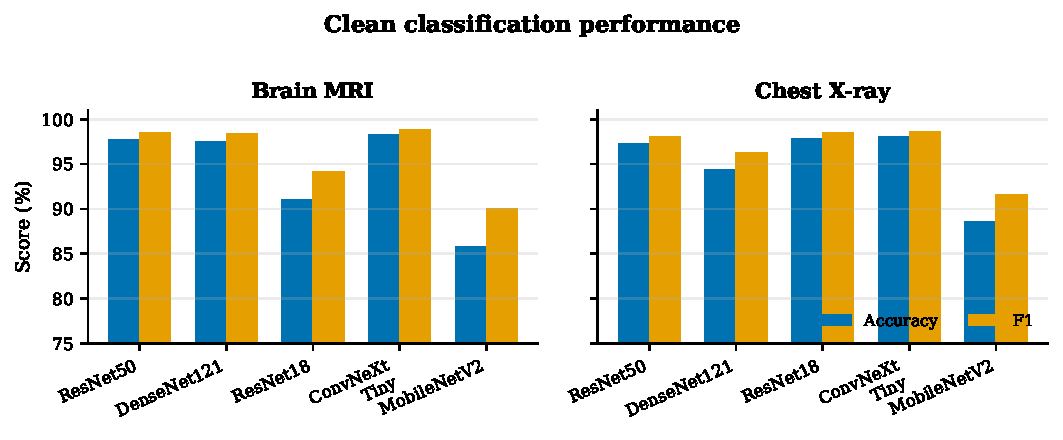
\includegraphics[width=\textwidth]{figures/clean_performance_overview.pdf}
  \caption{Clean accuracy and F1 for the five architectures on both medical classification tasks. Values are recomputed from the saved test predictions.}
  \label{fig:clean-performance-overview}
\end{figure}

The confusion matrices in Figure~\ref{fig:clean-confusion-matrices} expose error direction rather than only aggregate score. On brain MRI, ResNet50 produced 27 false tumour alarms but only four missed tumour cases, whereas ConvNeXt-Tiny reduced false positives to four while missing 19 tumour cases. MobileNetV2 made 156 false-negative tumour predictions, explaining why its sensitivity and F1 trail its precision. On chest X-ray, DenseNet121 missed only three pneumonia cases but classified 46 normal images as pneumonia; MobileNetV2 showed the opposite imbalance, with only three false positives but 97 missed pneumonia cases. These differences demonstrate that similar accuracy or AUC can conceal clinically different failure profiles.

\begin{figure}[htbp]
  \centering
  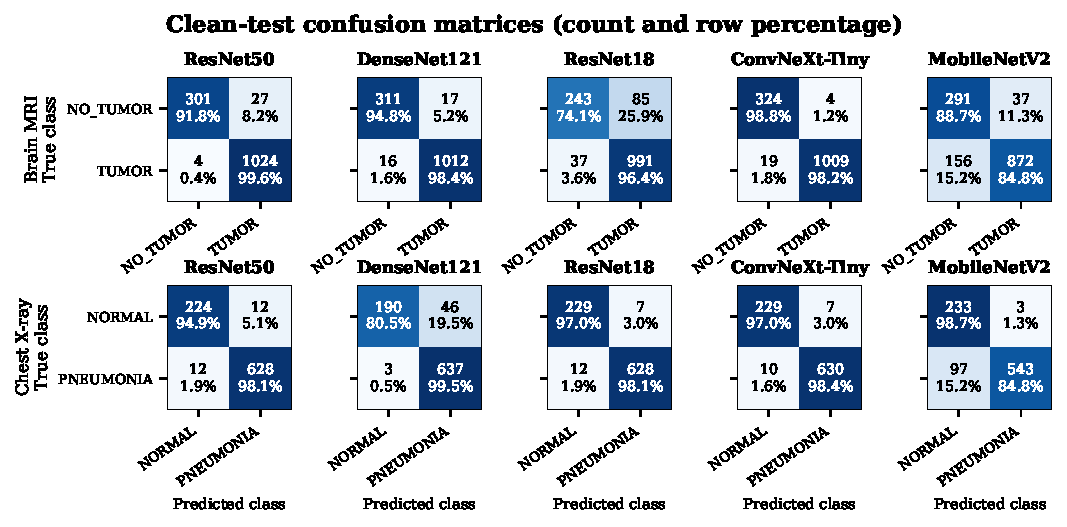
\includegraphics[width=\textwidth]{figures/clean_confusion_matrices.pdf}
  \caption{Clean-test confusion matrices for all five architectures on brain MRI ($n=1356$) and chest X-ray ($n=876$). Each cell reports the sample count and the percentage within its true class.}
  \label{fig:clean-confusion-matrices}
\end{figure}

\textbf{Sensitivity is especially relevant to the clinical interpretation of these experiments because it measures the proportion of positive cases that the classifier detects.} In this dissertation, the positive classes are TUMOR and PNEUMONIA, so $1-\mathrm{sensitivity}$ is the false-negative rate among affected cases. Figure~\ref{fig:clinical-sensitivity} shows that four models begin with clean sensitivity above 96\% on both tasks, whereas MobileNetV2 reaches only 84.82\% on each. This means that its lower aggregate performance is accompanied by a materially larger proportion of missed positive cases rather than only additional false alarms.

The attacked results change this clinical picture sharply. At $\epsilon=4/255$, ResNet50 retains 64.7\% of its clean brain MRI sensitivity under FGSM and 55.8\% under BIM, but only 8.5\% under PGD. DenseNet121 retains the most chest X-ray sensitivity under FGSM (37.4\%) and BIM (33.9\%), while every model retains at most 1.6\% under PGD. Thus an apparently accurate clean classifier can lose almost all ability to recognise the positive class under an iterative perturbation. Sensitivity must nevertheless be interpreted with specificity and precision: a model can obtain high recall by predicting the positive class too often, as illustrated by DenseNet121's 46 false-positive chest X-rays in Figure~\ref{fig:clean-confusion-matrices}.

\begin{figure}[htbp]
  \centering
  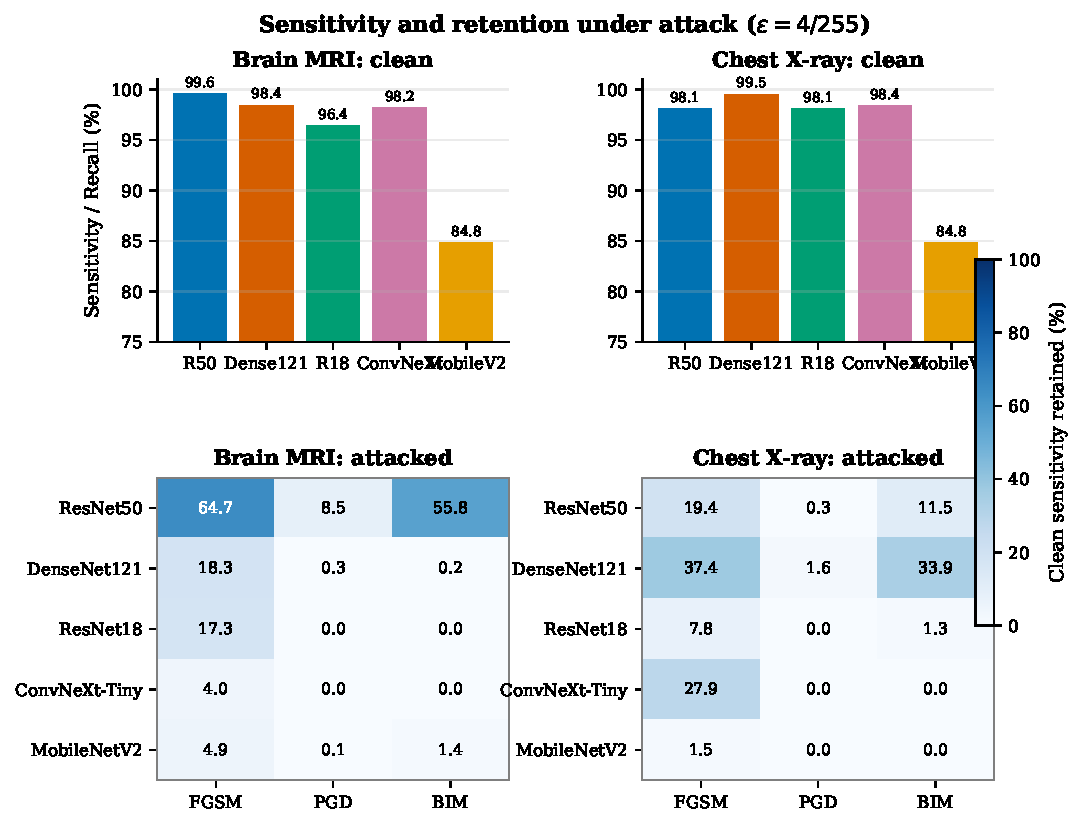
\includegraphics[width=\textwidth]{figures/clinical_sensitivity_summary.pdf}
  \caption{Clean sensitivity and the percentage of clean sensitivity retained under FGSM, PGD, and BIM at $\epsilon=4/255$. Sensitivity is recall for the positive clinical class (TUMOR or PNEUMONIA).}
  \label{fig:clinical-sensitivity}
\end{figure}

\noindent\textit{Key finding.} Clean performance alone does not identify a single uniformly superior architecture. ConvNeXt-Tiny leads both tasks, but the change in the middle of the ranking, especially ResNet18 moving from fourth on brain MRI to second on chest X-ray, shows that even standard generalisation depends on the image domain. The consistently high AUC values alongside larger differences in thresholded accuracy also indicate that ranking quality and operating-point performance should be considered separately.

\section{Within-Task Adversarial Robustness}
\label{sec:results-within-task}

\sectionfocus{Adversarial evaluation separates models far more sharply than clean testing and reveals different robustness leaders for brain MRI and chest X-ray.}

\subsection{Brain MRI}
\label{sec:results-brain}

Under FGSM, PGD, and BIM at $\epsilon = 4/255$ with ten iterative steps, robust accuracy on brain MRI varied widely across architectures (Table~\ref{tab:brain_mri_robustness_eps4}). ResNet50 retained the highest robust accuracy under every attack at this budget: 53.39\% (FGSM), 7.60\% (PGD), and 42.70\% (BIM). DenseNet121 fell to 22.27\%, 3.61\%, and 1.33\% respectively; MobileNetV2 to 15.19\%, 4.79\%, and 4.72\%; ResNet18 to 14.38\%, 0.00\%, and 0.00\%; and ConvNeXt-Tiny to 4.42\%, 0.00\%, and 0.00\%. ConvNeXt-Tiny and ResNet18 collapsed to 0\% robust accuracy under PGD and BIM from $\epsilon = 2/255$ onward despite leading or near-leading clean performance.

\begin{table}[htbp]
  \centering
  \caption{Adversarial accuracy (\%) of five standard models on Brain MRI at $\epsilon=4/255$.}
  \label{tab:brain_mri_robustness_eps4}
  \begin{tabular}{lrrr}
    \toprule
    Model & FGSM & PGD (steps=10) & BIM (steps=10) \\
    \midrule
    ResNet50        & 53.39 &  7.60 & 42.70 \\
    DenseNet121     & 22.27 &  3.61 &  1.33 \\
    ResNet18        & 14.38 &  0.00 &  0.00 \\
    ConvNeXt-Tiny   &  4.42 &  0.00 &  0.00 \\
    MobileNetV2     & 15.19 &  4.79 &  4.72 \\
    \bottomrule
  \end{tabular}
  \vspace{0.25em}
  \begin{minipage}{0.92\linewidth}
    \footnotesize
    PGD: random start, $\alpha=\epsilon/\text{steps}$, steps=10.
    BIM: no random start, $\alpha=\epsilon/\text{steps}$, steps=10.
  \end{minipage}
\end{table}

Table~\ref{tab:brain_mri_pgd_robustness_five_models} summarises PGD robustness across $\epsilon \in \{1,2,4\}/255$. ResNet50 degraded from 86.95\% at $\epsilon = 1/255$ to 61.28\% at $2/255$ and 7.60\% at $4/255$, with normalised R-AUC retention of 0.4782. DenseNet121 followed a similar but steeper curve (78.76\%, 38.94\%, 3.61\%; normalised R-AUC 0.4515). MobileNetV2 reached 30.68\%, 13.72\%, and 4.79\%, while ResNet18 and ConvNeXt-Tiny showed near-total collapse from $\epsilon = 1/255$ (robust accuracy 0.52\% and 0.22\% respectively). At $\epsilon = 2/255$, ResNet50 maintained 61.28\% robust accuracy with ASR 36.43\% and sensitivity retention 70.02\%; ConvNeXt-Tiny recorded ASR 98.30\% and 0\% robust accuracy under PGD and BIM. The non-linear decay between $\epsilon = 2/255$ and $4/255$ is particularly steep for ConvNeXt-Tiny and ResNet18, where a doubling of the budget erases residual robustness entirely, whereas ResNet50 retains a measurable 7.60\% band at $4/255$ before falling to 0\% at $8/255$. This pattern suggests that architecture selection for safety-critical MRI screening should prioritise performance at $\epsilon \ge 2/255$ under iterative attacks, not at the smallest budget alone where most models still exceed 30\% robust accuracy.

\begin{table}[htbp]
  \centering
  \caption{Core PGD robustness results on Brain MRI ($n=1356$, ten steps). Normalised R-AUC is the mean adversarial AUC retention over $\epsilon\in\{1,2,4\}/255$.}
  \label{tab:brain_mri_pgd_robustness_five_models}
  \begin{tabular}{lrrrrr}
    \toprule
    Model & Clean & Robust@1/255 & Robust@2/255 & Robust@4/255 & Norm. R-AUC \\
    \midrule
    ResNet50      & 97.71 & 86.95 & 61.28 & 7.60 & 0.4782 \\
    DenseNet121   & 97.57 & 78.76 & 38.94 & 3.61 & 0.4515 \\
    ResNet18      & 91.00 &  0.52 &  0.07 & 0.00 & 0.0006 \\
    ConvNeXt-Tiny & 98.30 &  0.22 &  0.00 & 0.00 & 0.0000 \\
    MobileNetV2   & 85.77 & 30.68 & 13.72 & 4.79 & 0.1980 \\
    \bottomrule
  \end{tabular}
  \vspace{0.25em}
  \begin{minipage}{0.88\linewidth}
    \footnotesize
    Clean and robust accuracy are reported in percent. ASR, sensitivity retention,
    and robust F1 at $2/255$ are reported in the accompanying text.
  \end{minipage}
\end{table}

Figure~\ref{fig:brain-pgd-models} makes the between-model decay easier to compare than the individual table entries. The separation is already visible at small budgets and becomes decisive by $\epsilon=2/255$.

\begin{figure}[htbp]
  \centering
  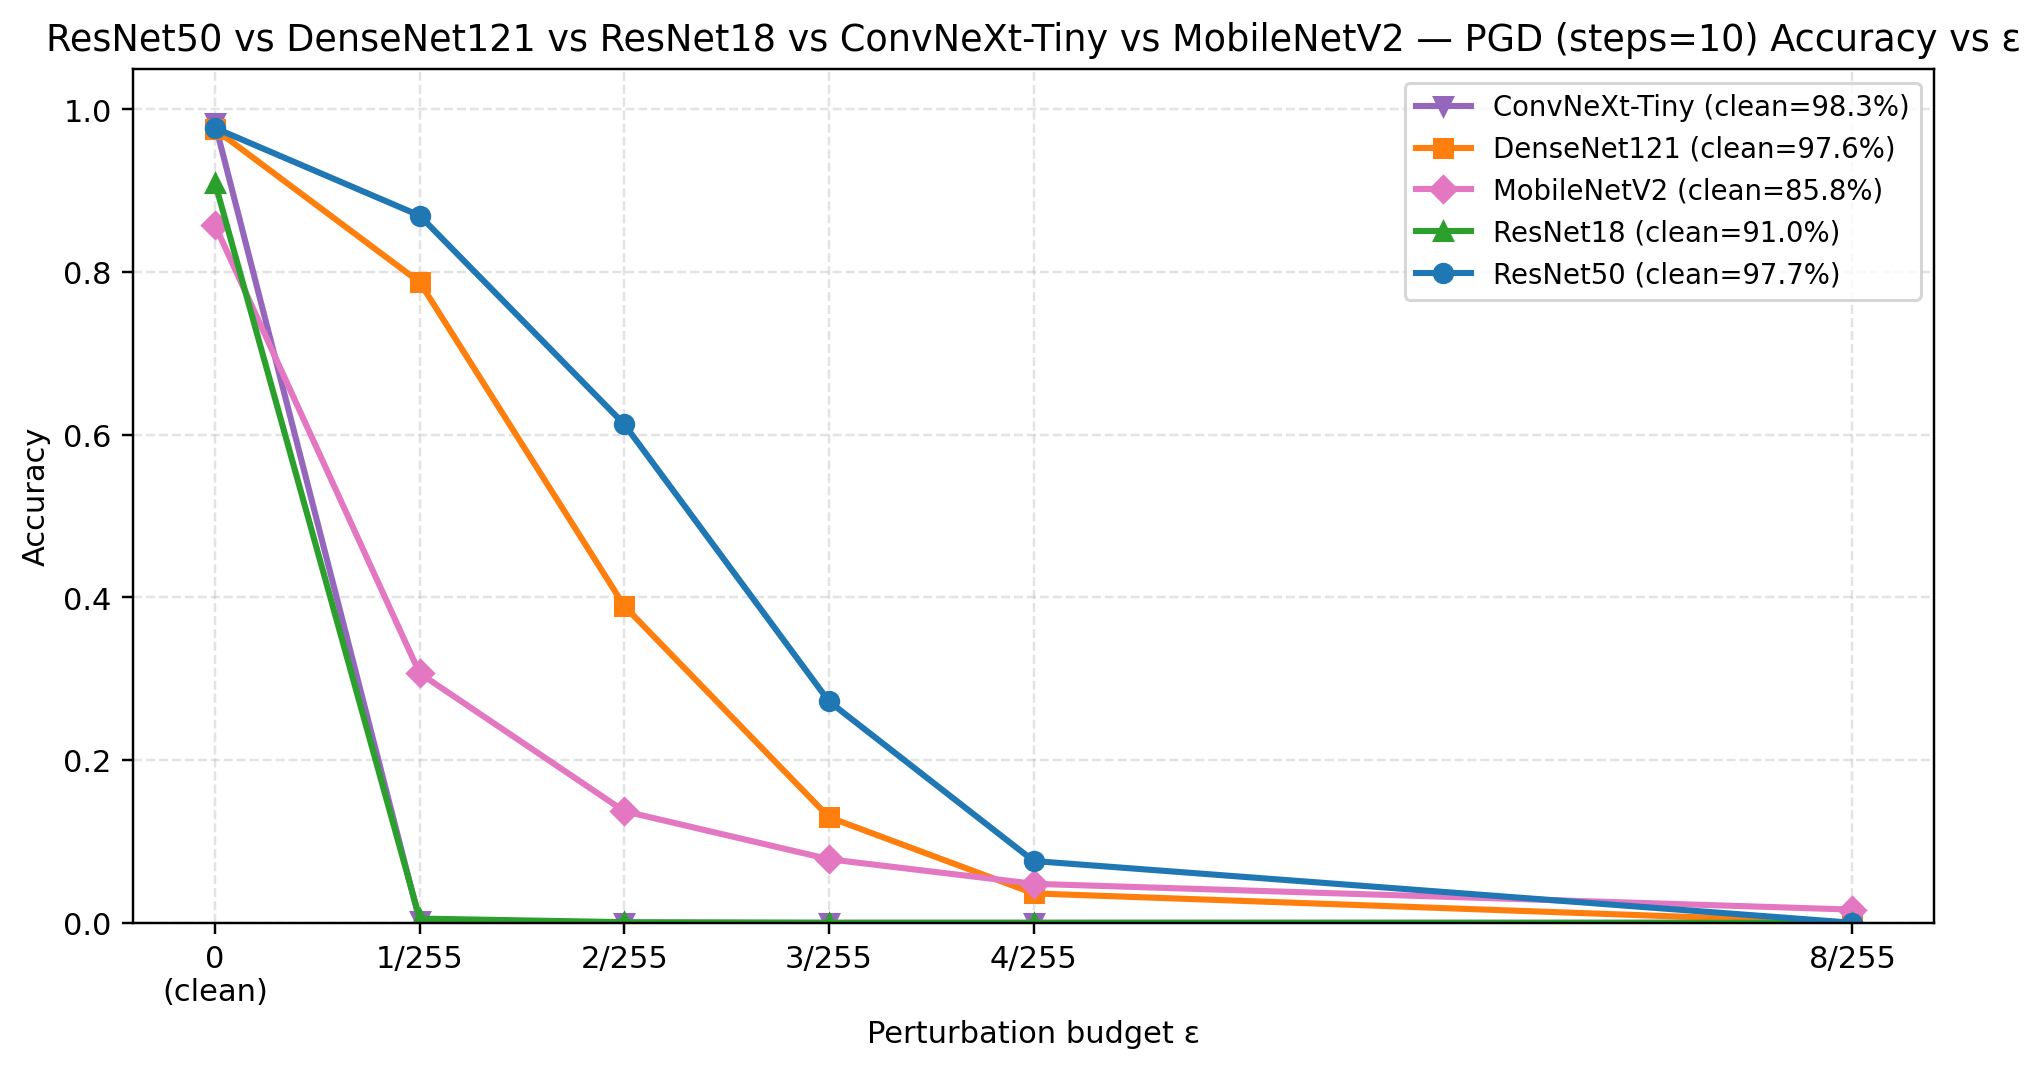
\includegraphics[width=0.88\textwidth]{figures/brain_mri_pgd_model_comparison.png}
  \caption{Brain MRI robust accuracy across PGD perturbation budgets for the five standard models. The plot complements Table~\ref{tab:brain_mri_pgd_robustness_five_models} by showing the shape of the degradation curves.}
  \label{fig:brain-pgd-models}
\end{figure}

\noindent\textit{Key finding.} On brain MRI, robustness separates the architectures much more sharply than clean accuracy. ResNet50 and DenseNet121 begin from similar clean baselines, yet ResNet50 retains 61.28\% PGD accuracy at $2/255$ compared with 38.94\% for DenseNet121. ConvNeXt-Tiny provides the clearest counterexample to selecting a model from the clean leaderboard: its 98.30\% clean accuracy falls to zero at the same budget.

\subsection{Chest X-ray}
\label{sec:results-chest}

On chest X-ray at $\epsilon = 4/255$, robustness patterns differed from brain MRI. Under PGD (steps=10), ResNet50 robust accuracy was 0.23\% (ASR 97.03\%), DenseNet121 1.14\% (ASR 93.26\%), ResNet18 0.00\%, ConvNeXt-Tiny 0.00\%, and MobileNetV2 0.00\%. Under FGSM at the same budget, ResNet50 retained 13.93\%, DenseNet121 27.17\%, ConvNeXt-Tiny 22.26\%, ResNet18 5.59\%, and MobileNetV2 0.91\%. Under BIM, ResNet50 reached 8.22\%, DenseNet121 24.66\%, and all other models 0.00\% or 0.91\%. DenseNet121 therefore showed the highest FGSM and BIM robust accuracy on chest X-ray at $\epsilon = 4/255$, whereas ResNet50 was most robust on brain MRI under the same attacks, indicating that architecture rankings are task-dependent.

At $\epsilon = 2/255$ on chest X-ray, PGD robust accuracy was ResNet50 18.04\%, DenseNet121 31.85\%, ConvNeXt-Tiny 0.00\%, ResNet18 0.34\%, and MobileNetV2 0.00\%. FGSM robust accuracy at $\epsilon = 2/255$ was DenseNet121 42.35\%, ConvNeXt-Tiny 29.57\%, ResNet50 27.05\%, ResNet18 13.47\%, and MobileNetV2 0.91\%.

Figure~\ref{fig:all-robustness-curves} uses every recorded perturbation budget rather than selecting only $2/255$ and $4/255$. Three additional patterns emerge. First, the degradation is strongly non-linear: several models collapse between $1/255$ and $2/255$, so reporting only the largest budget would hide the transition point. Second, FGSM curves usually decline more gradually than PGD and BIM, confirming that a single-step evaluation gives an optimistic view of robustness. Third, ResNet50's unusually flat BIM tail on brain MRI contrasts with DenseNet121's rapid BIM collapse, while DenseNet121 retains the clearest advantage on chest X-ray. Thus both the ordering and the shape of degradation are architecture--task interactions.

\begin{figure}[htbp]
  \centering
  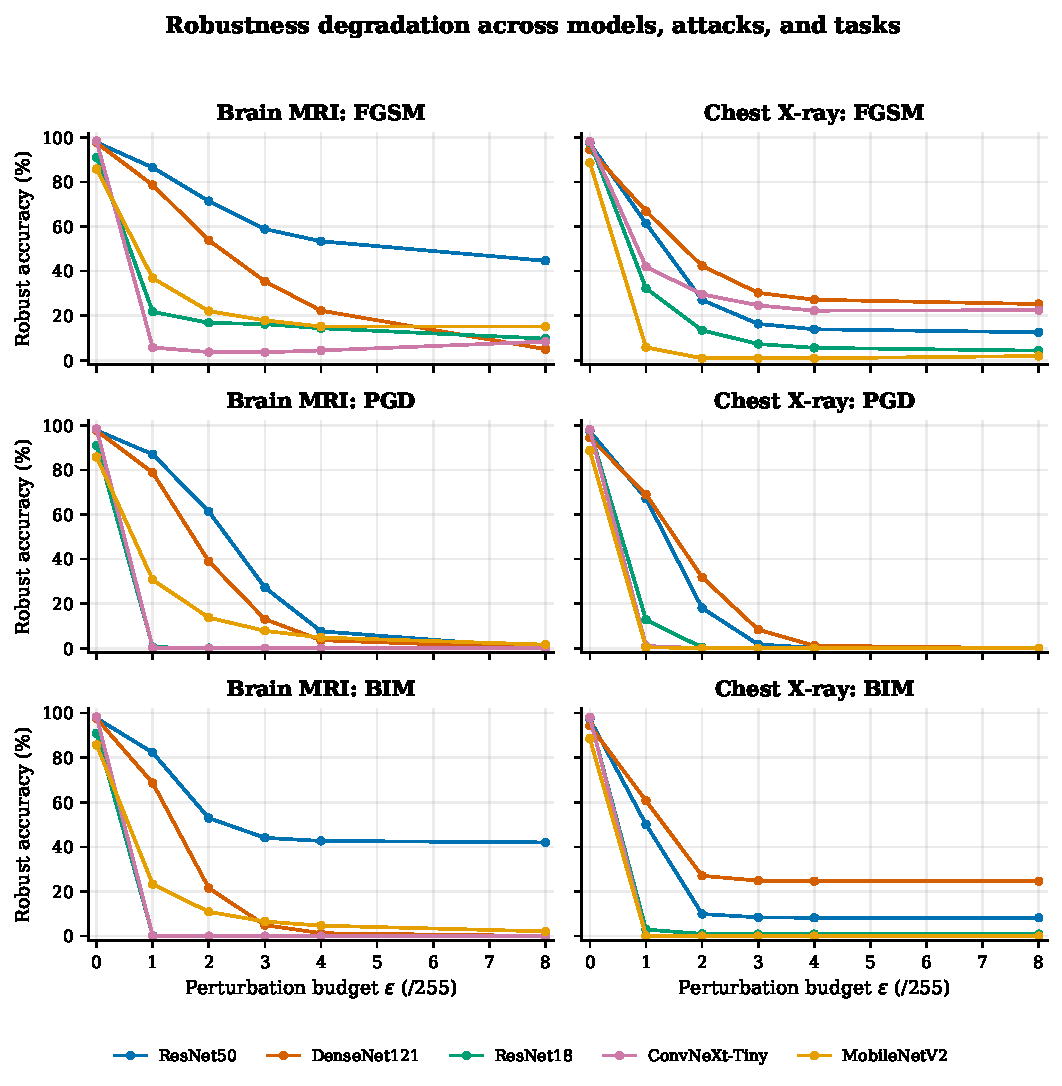
\includegraphics[width=\textwidth]{figures/adversarial_robustness_curves.pdf}
  \caption{Robust accuracy across the full recorded perturbation range for five models, three attacks, and two tasks. Iterative PGD and BIM use ten steps.}
  \label{fig:all-robustness-curves}
\end{figure}

The heatmaps in Figure~\ref{fig:robustness-heatmaps} provide a fixed-budget view of the same interaction. At $4/255$, only ResNet50 retains more than 40\% accuracy under two brain MRI attacks, while DenseNet121 is the only chest X-ray model above 20\% under both FGSM and BIM. The concentration of near-zero cells under PGD shows that the clean leaderboard has little discriminatory value once the iterative attack reaches this budget.

\begin{figure}[htbp]
  \centering
  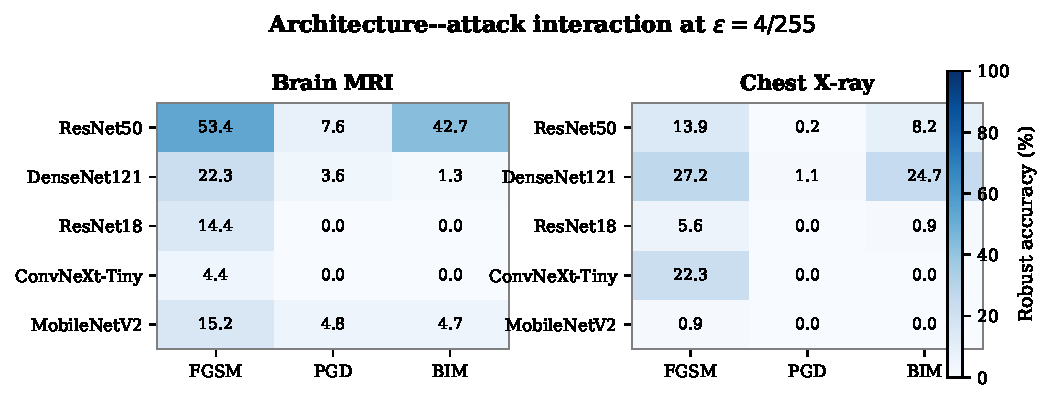
\includegraphics[width=0.94\textwidth]{figures/robustness_heatmaps_eps4.pdf}
  \caption{Architecture--attack interaction at $\epsilon=4/255$. Cell values are robust accuracy (\%); darker cells indicate greater retained accuracy.}
  \label{fig:robustness-heatmaps}
\end{figure}

\noindent\textit{Key finding.} The chest X-ray task is not simply a lower-scoring copy of the brain MRI experiment. DenseNet121 becomes the strongest model under PGD, FGSM, and BIM at the reported budgets, while the clean leader again fails under iterative attacks. This reversal answers the second research question provisionally: architecture-level robustness does not transfer reliably between the two tasks.

\section{Cross-Task Comparisons}
\label{sec:results-cross-task}

\sectionfocus{Absolute robustness and architecture rankings are task-dependent, whereas the broad distinction between weaker single-step and stronger iterative attacks is more stable.}

Cross-task differences were computed at matched $\epsilon$ values for each architecture and attack. Table~\ref{tab:cross_task_eps4} reports robust accuracy at $\epsilon = 4/255$ under PGD (steps=10) on both tasks. ResNet50 robust accuracy fell from 7.60\% (brain MRI) to 0.23\% (chest X-ray), a cross-task gap $\Delta_{\mathrm{robust}} = +7.37$ percentage points in favour of brain MRI. DenseNet121 fell from 3.61\% to 1.14\% ($\Delta = +2.47$). ConvNeXt-Tiny, ResNet18, and MobileNetV2 recorded 0\% under PGD on both tasks at this budget. Under FGSM at $\epsilon = 4/255$, ResNet50 dropped from 53.39\% to 13.93\% ($\Delta = +39.46$), and DenseNet121 from 22.27\% to 27.17\% ($\Delta = -4.90$), reversing the brain MRI ordering.

\begin{table}[htbp]
  \centering
  \caption{Cross-task robust accuracy (\%) at $\epsilon = 4/255$ under PGD (steps=10).}
  \label{tab:cross_task_eps4}
  \begin{tabular}{lrrr}
    \toprule
    Model & Brain MRI & Chest X-ray & $\Delta_{\mathrm{robust}}$ \\
    \midrule
    ResNet50       &  7.60 &  0.23 & $+$7.37 \\
    DenseNet121    &  3.61 &  1.14 & $+$2.47 \\
    ResNet18       &  0.00 &  0.00 &  0.00 \\
    ConvNeXt-Tiny  &  0.00 &  0.00 &  0.00 \\
    MobileNetV2    &  4.79 &  0.00 & $+$4.79 \\
    \bottomrule
  \end{tabular}
\end{table}

The comparison in Figure~\ref{fig:chest-pgd-models} shows that the chest X-ray curves do not simply reproduce the brain MRI ordering. In particular, DenseNet121 retains more accuracy than ResNet50 at the intermediate budgets, while several models reach the floor early.

\begin{figure}[htbp]
  \centering
  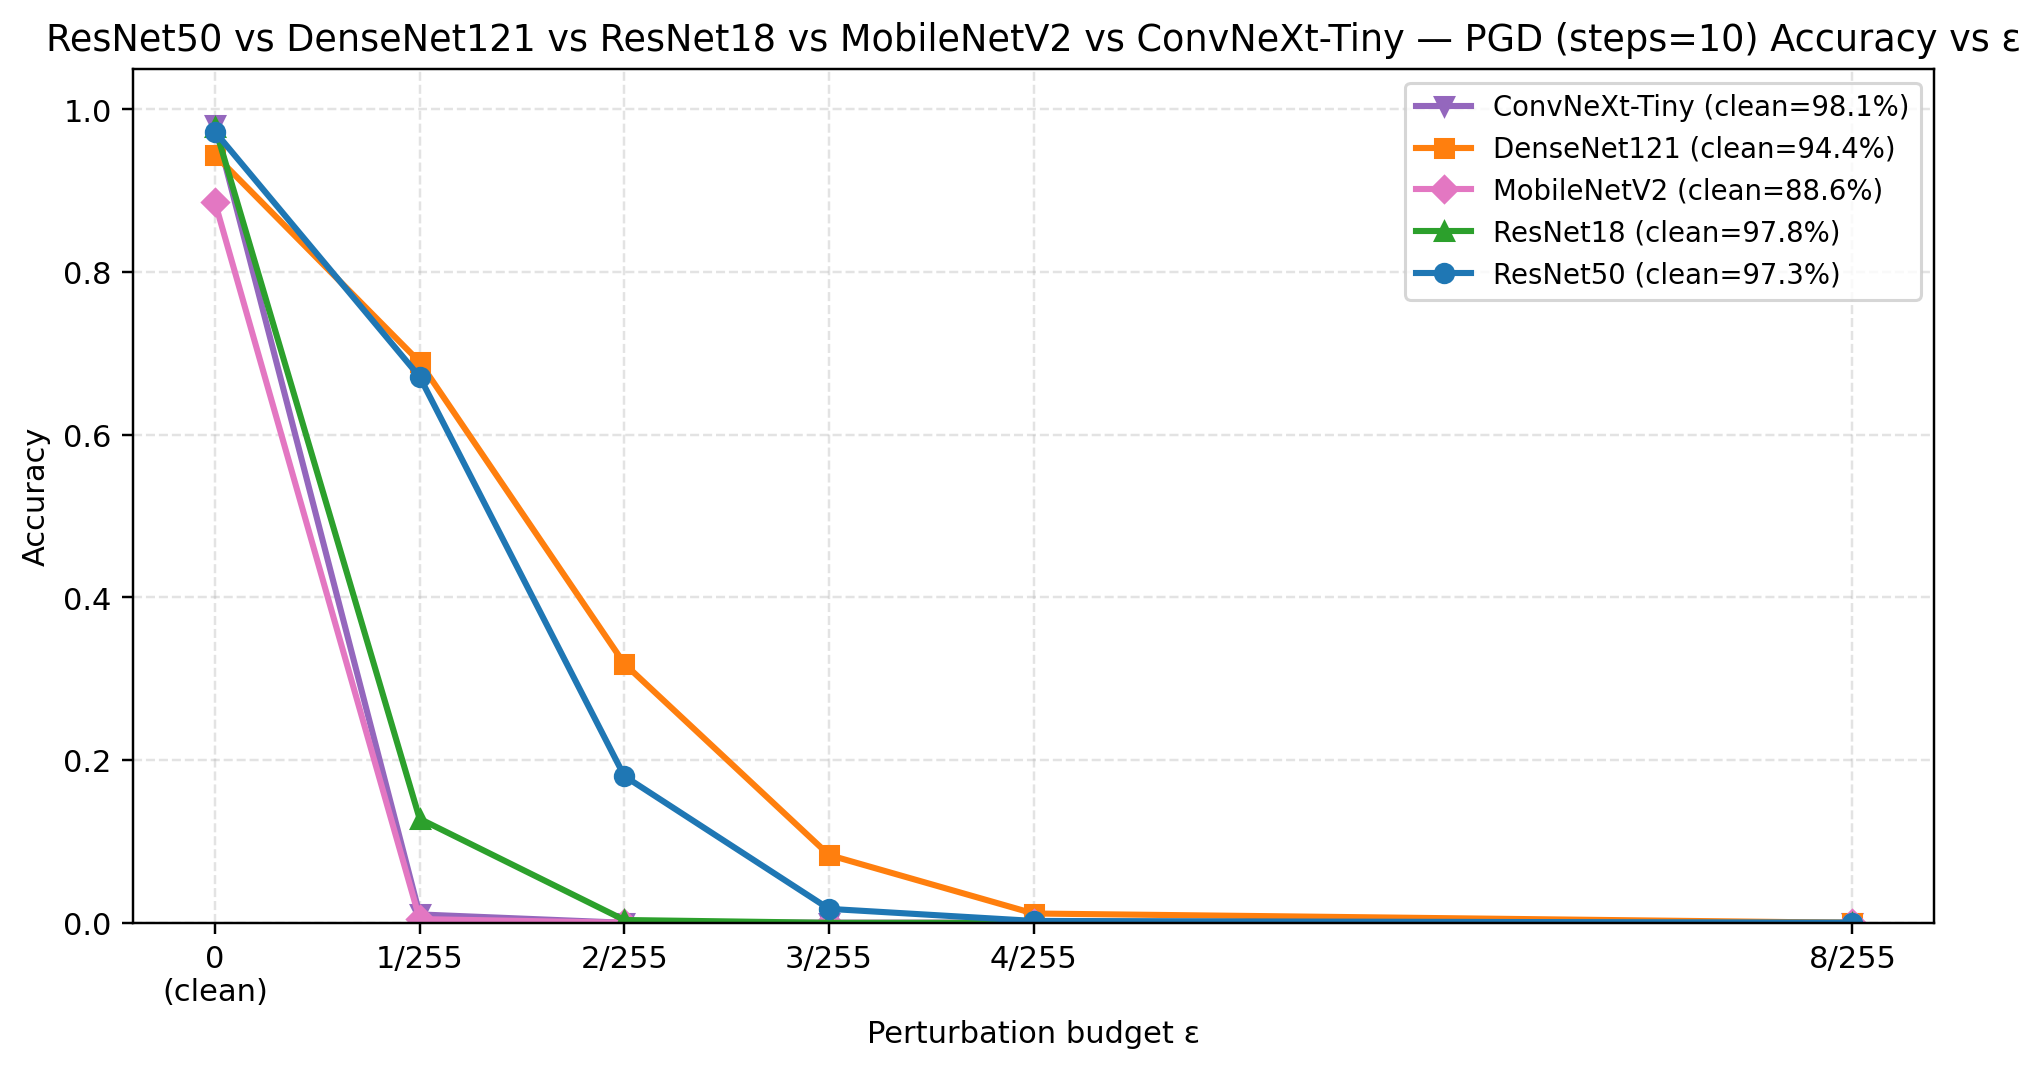
\includegraphics[width=0.88\textwidth]{figures/chest_xray_pgd_model_comparison.png}
  \caption{Chest X-ray robust accuracy across PGD perturbation budgets for the five standard models.}
  \label{fig:chest-pgd-models}
\end{figure}

\subsection{ResNet50 attack-strength comparison ($L_\infty$ family)}
\label{sec:results-r50-attack-strength}

Attack-strength analysis fixes the reference architecture to ResNet50 and ranks FGSM, PGD, BIM, and MIM under a common white-box $L_\infty$ protocol (ten steps for iterative attacks; MIM with momentum $\mu = 1.0$). Lower robust accuracy and higher attack success rate (ASR) indicate a stronger attack at a fixed budget~$\epsilon$. Table~\ref{tab:r50_attack_strength} reports results at $\epsilon = 2/255$ and $4/255$ on both tasks.

On brain MRI, the attack-strength ordering was consistent across both budgets: FGSM was weakest and MIM strongest. At $\epsilon = 4/255$, robust accuracy ranked FGSM (53.39\%) $>$ BIM (42.70\%) $>$ PGD (7.60\%) $>$ MIM (1.22\%), with ASR 44.32\%, 55.01\%, 90.12\%, and 98.78\% respectively. At $\epsilon = 2/255$, the ordering was FGSM (71.39\%) $>$ PGD (61.28\%) $>$ BIM (52.95\%) $>$ MIM (14.63\%). On chest X-ray, the same relative ordering held at $\epsilon = 4/255$: FGSM (13.93\%) $>$ BIM (8.22\%) $>$ PGD (0.23\%) $>$ MIM (0.11\%), with ASR 83.33\%, 89.04\%, 97.03\%, and 99.89\%. At $\epsilon = 2/255$ on chest X-ray, FGSM (27.05\%) remained weakest while PGD (18.04\%) exceeded BIM (9.93\%) and MIM (9.59\%) in robust accuracy; MIM still recorded the highest ASR (90.41\%). Absolute robust accuracy under every attack was lower on chest X-ray than on brain MRI, but the dominance of MIM and PGD over FGSM transferred across both domains.

\begin{table}[htbp]
  \centering
  \caption{ResNet50 attack-strength summary under the unified $L_\infty$ protocol. Robust accuracy (\%) and ASR (\%) at $\epsilon = 2/255$ and $4/255$; iterative attacks use ten steps.}
  \label{tab:r50_attack_strength}
  \small
  \begin{tabular}{llrrrr}
    \toprule
    Task & Attack & \multicolumn{2}{c}{$\epsilon = 2/255$} & \multicolumn{2}{c}{$\epsilon = 4/255$} \\
    \cmidrule(lr){3-4} \cmidrule(lr){5-6}
    & & Robust Acc. & ASR & Robust Acc. & ASR \\
    \midrule
    \multirow{4}{*}{Brain MRI}
      & FGSM & 71.39 & 26.33 & 53.39 & 44.32 \\
      & PGD  & 61.28 & 36.43 &  7.60 & 90.12 \\
      & BIM  & 52.95 & 44.76 & 42.70 & 55.01 \\
      & MIM  & 14.63 & 85.37 &  1.22 & 98.78 \\
    \midrule
    \multirow{4}{*}{Chest X-ray}
      & FGSM & 27.05 & 70.21 & 13.93 & 83.33 \\
      & PGD  & 18.04 & 79.22 &  0.23 & 97.03 \\
      & BIM  &  9.93 & 87.33 &  8.22 & 89.04 \\
      & MIM  &  9.59 & 90.41 &  0.11 & 99.89 \\
    \bottomrule
  \end{tabular}
  \vspace{0.25em}
  \begin{minipage}{0.92\linewidth}
    \footnotesize
    Clean accuracy: Brain MRI 97.71\%; Chest X-ray 97.26\%.
    MIM evaluated on ResNet50 only (by design).
    Attack strength increases as robust accuracy decreases (ASR increases).
  \end{minipage}
\end{table}

Figure~\ref{fig:r50-attack-strength-bars} shows both budgets without mixing robust accuracy with ASR in the same axis. Increasing the budget from $2/255$ to $4/255$ reduces brain MRI PGD accuracy by 53.68 percentage points and MIM accuracy by 13.41 points. On chest X-ray, the remaining margin is already small at $2/255$, and PGD and MIM approach zero at $4/255$. BIM is an exception to a simple monotonic ranking: it is more damaging than PGD at $2/255$ but less damaging at $4/255$ on both tasks, illustrating why attack-strength claims must specify the perturbation budget.

\begin{figure}[htbp]
  \centering
  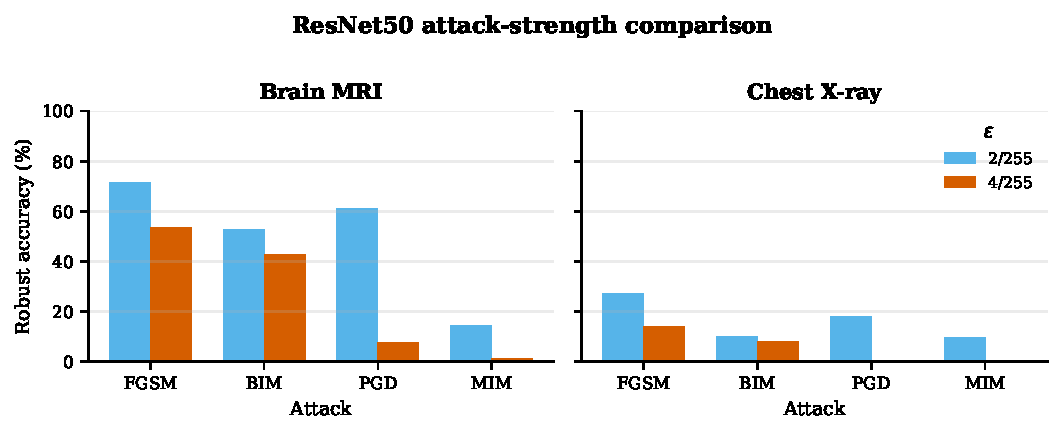
\includegraphics[width=\textwidth]{figures/resnet50_attack_strength_comparison.pdf}
  \caption{ResNet50 robust accuracy under FGSM, BIM, PGD, and MIM at two matched perturbation budgets on both tasks. Lower bars indicate stronger attacks.}
  \label{fig:r50-attack-strength-bars}
\end{figure}

\noindent\textit{Key finding.} Absolute robustness varies substantially by task, but the attack comparison is more stable than the model comparison. On ResNet50, iterative attacks with momentum or random initialisation are consistently more damaging than FGSM at $4/255$. A single FGSM result would therefore overstate robustness on both datasets, even though the precise ordering of PGD and BIM changes at the smaller budget.

\section{Defence Experiments on Brain MRI}
\label{sec:results-defence}

\sectionfocus{PGD adversarial training provides the largest individual robustness gain, and combining it with Gaussian smoothing produces the strongest evaluated defence.}

PGD adversarial training (PGD-AT) was applied to ResNet50 and DenseNet121 on brain MRI with $\epsilon_{\mathrm{train}} = 4/255$ and ten inner steps. Under PGD evaluation (steps=10), standard ResNet50 robust accuracy progressed from 86.95\% at $\epsilon = 1/255$ to 61.28\%, 27.21\%, 7.60\%, and 0.00\% at $\epsilon = 2/255$, $3/255$, $4/255$, and $8/255$ respectively; PGD-AT ResNet50 achieved 98.53\%, 97.35\%, 94.76\%, 89.38\%, and 34.07\% at the same budgets (Table~\ref{tab:pgd_at_pgd_steps10}). Standard DenseNet121 degraded from 78.76\% at $\epsilon = 1/255$ to 38.94\%, 12.98\%, 3.61\%, and 0.00\% at $\epsilon = 2/255$, $3/255$, $4/255$, and $8/255$; PGD-AT DenseNet121 maintained 97.64\%, 94.76\%, 88.42\%, and 30.16\% at $\epsilon = 2/255$, $3/255$, $4/255$, and $8/255$.

\begin{table}[htbp]
  \centering
  \caption{Standard vs.\ PGD-AT accuracy (\%) under PGD attack (steps=10) on Brain MRI.}
  \label{tab:pgd_at_pgd_steps10}
  \begin{tabular}{llrrrrr}
    \toprule
    Model & Variant & $\epsilon=1/255$ & $2/255$ & $3/255$ & $4/255$ & $8/255$ \\
    \midrule
    \multirow{2}{*}{ResNet50}
      & Standard & 86.95 & 61.28 & 27.21 &  7.60 &  0.00 \\
      & PGD-AT   & 98.53 & 97.35 & 94.76 & 89.38 & 34.07 \\
    \midrule
    \multirow{2}{*}{DenseNet121}
      & Standard & 78.76 & 38.94 & 12.98 &  3.61 &  0.00 \\
      & PGD-AT   & 98.16 & 97.64 & 94.76 & 88.42 & 30.16 \\
    \bottomrule
  \end{tabular}
  \vspace{0.25em}
  \begin{minipage}{0.92\linewidth}
    \footnotesize
    PGD-AT training: $\epsilon_{\train}=4/255$, PGD steps=10, mix\_clean=0.5.
    PGD evaluation: random start, steps=10, $\alpha=\epsilon/\text{steps}$.
    Standard DenseNet121 PGD values are from the five-model benchmark (Table~\ref{tab:brain_mri_pgd_robustness_five_models}).
  \end{minipage}
\end{table}

Figure~\ref{fig:pgd-at-curve} visualises the central defence result: adversarial training changes the full degradation curve rather than improving a single operating point. The advantage narrows at $8/255$, which is obscured when attention is restricted to the $4/255$ column.

\begin{figure}[htbp]
  \centering
  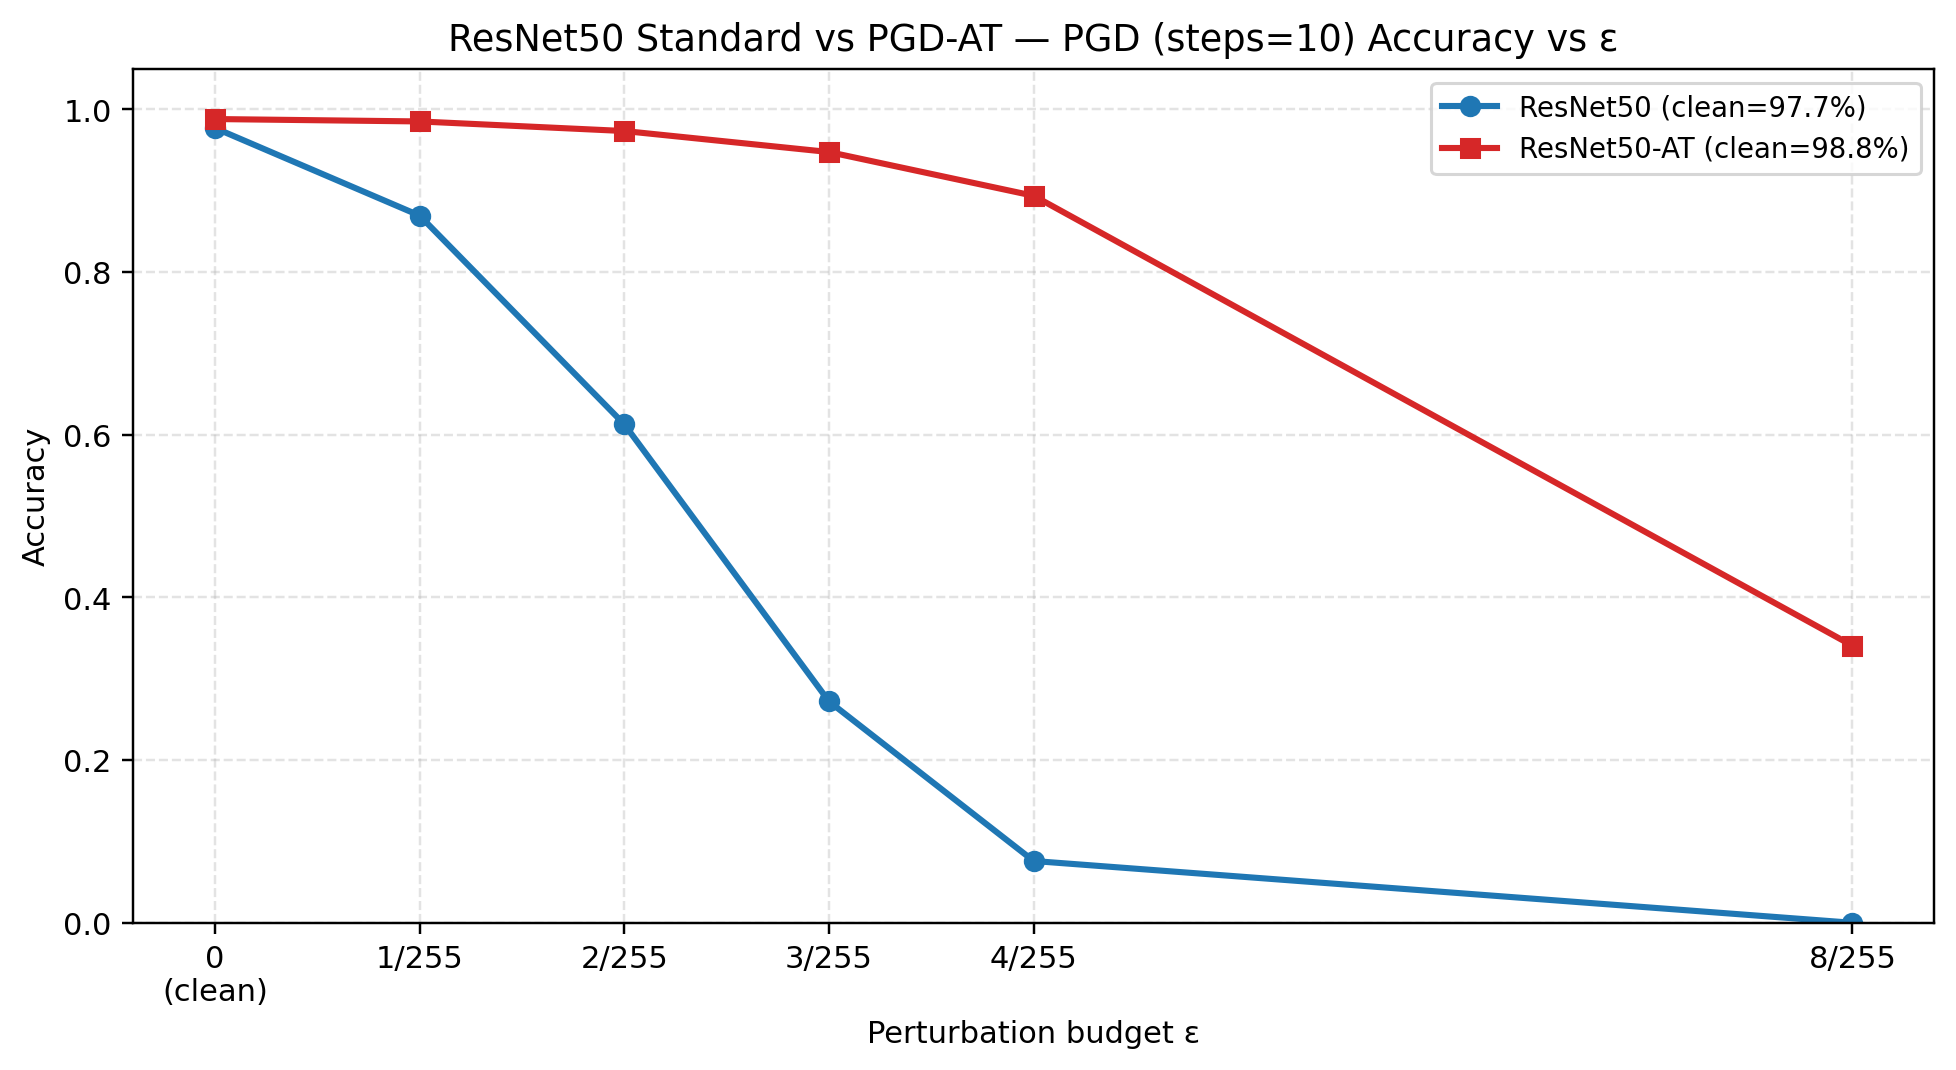
\includegraphics[width=0.88\textwidth]{figures/brain_mri_pgd_standard_vs_at.png}
  \caption{ResNet50 accuracy under PGD for standard and PGD-adversarially trained models on brain MRI (ten attack steps).}
  \label{fig:pgd-at-curve}
\end{figure}

At $\epsilon = 4/255$, cross-attack evaluation confirmed that PGD-AT improved robustness under attacks not seen identically during training (Table~\ref{tab:pgd_at_cross_attack_eps4}). PGD-AT ResNet50 reached 89.38\% under PGD, 80.24\% under BIM, and 90.71\% under FGSM, compared with 7.60\%, 42.70\%, and 53.39\% for the standard model. PGD-AT DenseNet121 reached 88.42\%, 77.58\%, and 89.53\% under PGD, BIM, and FGSM, compared with 3.61\%, 1.33\%, and 22.27\% for the standard model. The cross-attack transfer is asymmetric: FGSM robust accuracy under PGD-AT exceeds PGD robust accuracy at the same $\epsilon$ for both architectures (ResNet50 FGSM 90.71\% versus PGD 89.38\%), because single-step attacks remain weaker even against adversarially trained weights. Under BIM across the full $\epsilon$ sweep, PGD-AT ResNet50 maintained above 80\% robust accuracy through $\epsilon = 4/255$ (80.24\%) before falling to 19.54\% at $\epsilon = 8/255$; PGD-AT DenseNet121 showed a similar profile (77.58\% at $\epsilon = 4/255$, 16.67\% at $8/255$). These results indicate that PGD-AT generalises beyond the exact inner-loop attack used during training, though large budgets ($\epsilon = 8/255$) remain a stress test for both standard and hardened models.

\begin{table}[htbp]
  \centering
  \caption{Standard vs.\ PGD-AT accuracy (\%) under three attacks at $\epsilon=4/255$ (Brain MRI).}
  \label{tab:pgd_at_cross_attack_eps4}
  \begin{tabular}{llrrr}
    \toprule
    Model & Variant & PGD & BIM & FGSM \\
    \midrule
    \multirow{2}{*}{ResNet50}
      & Standard &  7.60 & 42.70 & 53.39 \\
      & PGD-AT   & 89.38 & 80.24 & 90.71 \\
    \midrule
    \multirow{2}{*}{DenseNet121}
      & Standard &  3.61 &  1.33 & 22.27 \\
      & PGD-AT   & 88.42 & 77.58 & 89.53 \\
    \bottomrule
  \end{tabular}
  \vspace{0.25em}
  \begin{minipage}{0.92\linewidth}
    \footnotesize
    PGD/BIM evaluation uses steps=10.
    PGD-AT models were trained with PGD at $\epsilon_{\train}=4/255$.
  \end{minipage}
\end{table}

The four-condition Gaussian smoothing protocol on ResNet50 evaluated inference-time blur alone and combined with PGD-AT (Table~\ref{tab:gaussian_defense_resnet50}). Condition D0 (standard model, no blur) yielded clean accuracy 97.71\% and PGD robust accuracy 61.21\% at $\epsilon = 2/255$, falling to 7.52\% at $\epsilon = 4/255$; BIM robust accuracy was 52.95\% and 42.70\% at the same budgets. Condition D1 (blur on adversarial inputs only) raised PGD robust accuracy to 79.13\% and 50.59\%, and BIM to 79.35\% and 58.63\%, without changing clean accuracy. Condition D2 (blur on all inputs) produced identical adversarial metrics to D1 but reduced clean accuracy to 93.95\%. Condition D3 (all-input blur with PGD-AT ResNet50) achieved clean accuracy 98.53\% and PGD robust accuracy 97.64\% at $\epsilon = 2/255$ and 96.53\% at $\epsilon = 4/255$; BIM robust accuracy under D3 was 97.49\% and 96.09\% at $\epsilon = 2/255$ and $4/255$ respectively.

\begin{table}[htbp]
  \centering
  \caption{Gaussian smoothing defence on ResNet50 (Brain MRI). Accuracy (\%) under ten-step PGD and BIM; blur radius $\sigma=1.0$.}
  \label{tab:gaussian_defense_resnet50}
  \begin{tabular}{llrrrrr}
    \toprule
    & & & \multicolumn{2}{c}{$\epsilon=2/255$} & \multicolumn{2}{c}{$\epsilon=4/255$} \\
    \cmidrule(lr){4-5} \cmidrule(lr){6-7}
    Cond. & Setting & Clean & PGD & BIM & PGD & BIM \\
    \midrule
    D0 & No defence          & 97.71 & 61.21 & 52.95 &  7.52 & 42.70 \\
    D1 & Adversarial-only blur & 97.71 & 79.13 & 79.35 & 50.59 & 58.63 \\
    D2 & All-input blur      & 93.95 & 79.13 & 79.35 & 50.59 & 58.63 \\
    D3 & PGD-AT + all-input blur & 98.53 & 97.64 & 97.49 & 96.53 & 96.09 \\
    \bottomrule
  \end{tabular}
  \vspace{0.25em}
  \begin{minipage}{0.92\linewidth}
    \footnotesize
    D0: no preprocessing. D1: Gaussian blur on adversarial inputs only.
    D2: blur on all inputs (Standard ResNet50).
    D3: blur on all inputs with PGD-AT ResNet50 (trained at $\epsilon_{\train}=4/255$, steps=10).
    PGD uses random start; BIM has no random start; $\alpha=\epsilon/\text{steps}$.
  \end{minipage}
\end{table}

Figure~\ref{fig:pgd-at-cross-attack} makes the transfer of the training-time defence explicit. For ResNet50, PGD-AT adds 37.32 percentage points under FGSM, 81.78 under PGD, and 37.54 under BIM at $4/255$. The corresponding gains for DenseNet121 are 67.26, 84.81, and 76.25 points. The largest improvements occur where the standard networks were weakest, but the defended FGSM, PGD, and BIM results converge to a relatively narrow 77.58--90.71\% band. This reduces attack-specific variation as well as increasing mean robustness.

\begin{figure}[htbp]
  \centering
  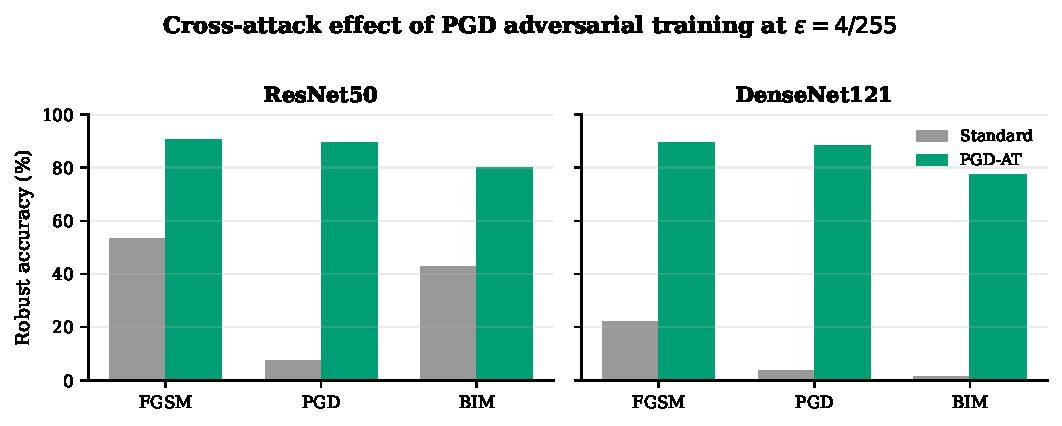
\includegraphics[width=\textwidth]{figures/pgd_at_cross_attack_eps4.pdf}
  \caption{Cross-attack robust accuracy of standard and PGD-adversarially trained ResNet50 and DenseNet121 at $\epsilon=4/255$ on brain MRI.}
  \label{fig:pgd-at-cross-attack}
\end{figure}

Figure~\ref{fig:gaussian-factorial} emphasises the factorial comparison at $\epsilon=4/255$. D1 and D2 share the same adversarial accuracy because their attack-time transformation is identical; their practical difference appears in clean performance and whether oracle knowledge of adversarial inputs is assumed.

\begin{figure}[htbp]
  \centering
  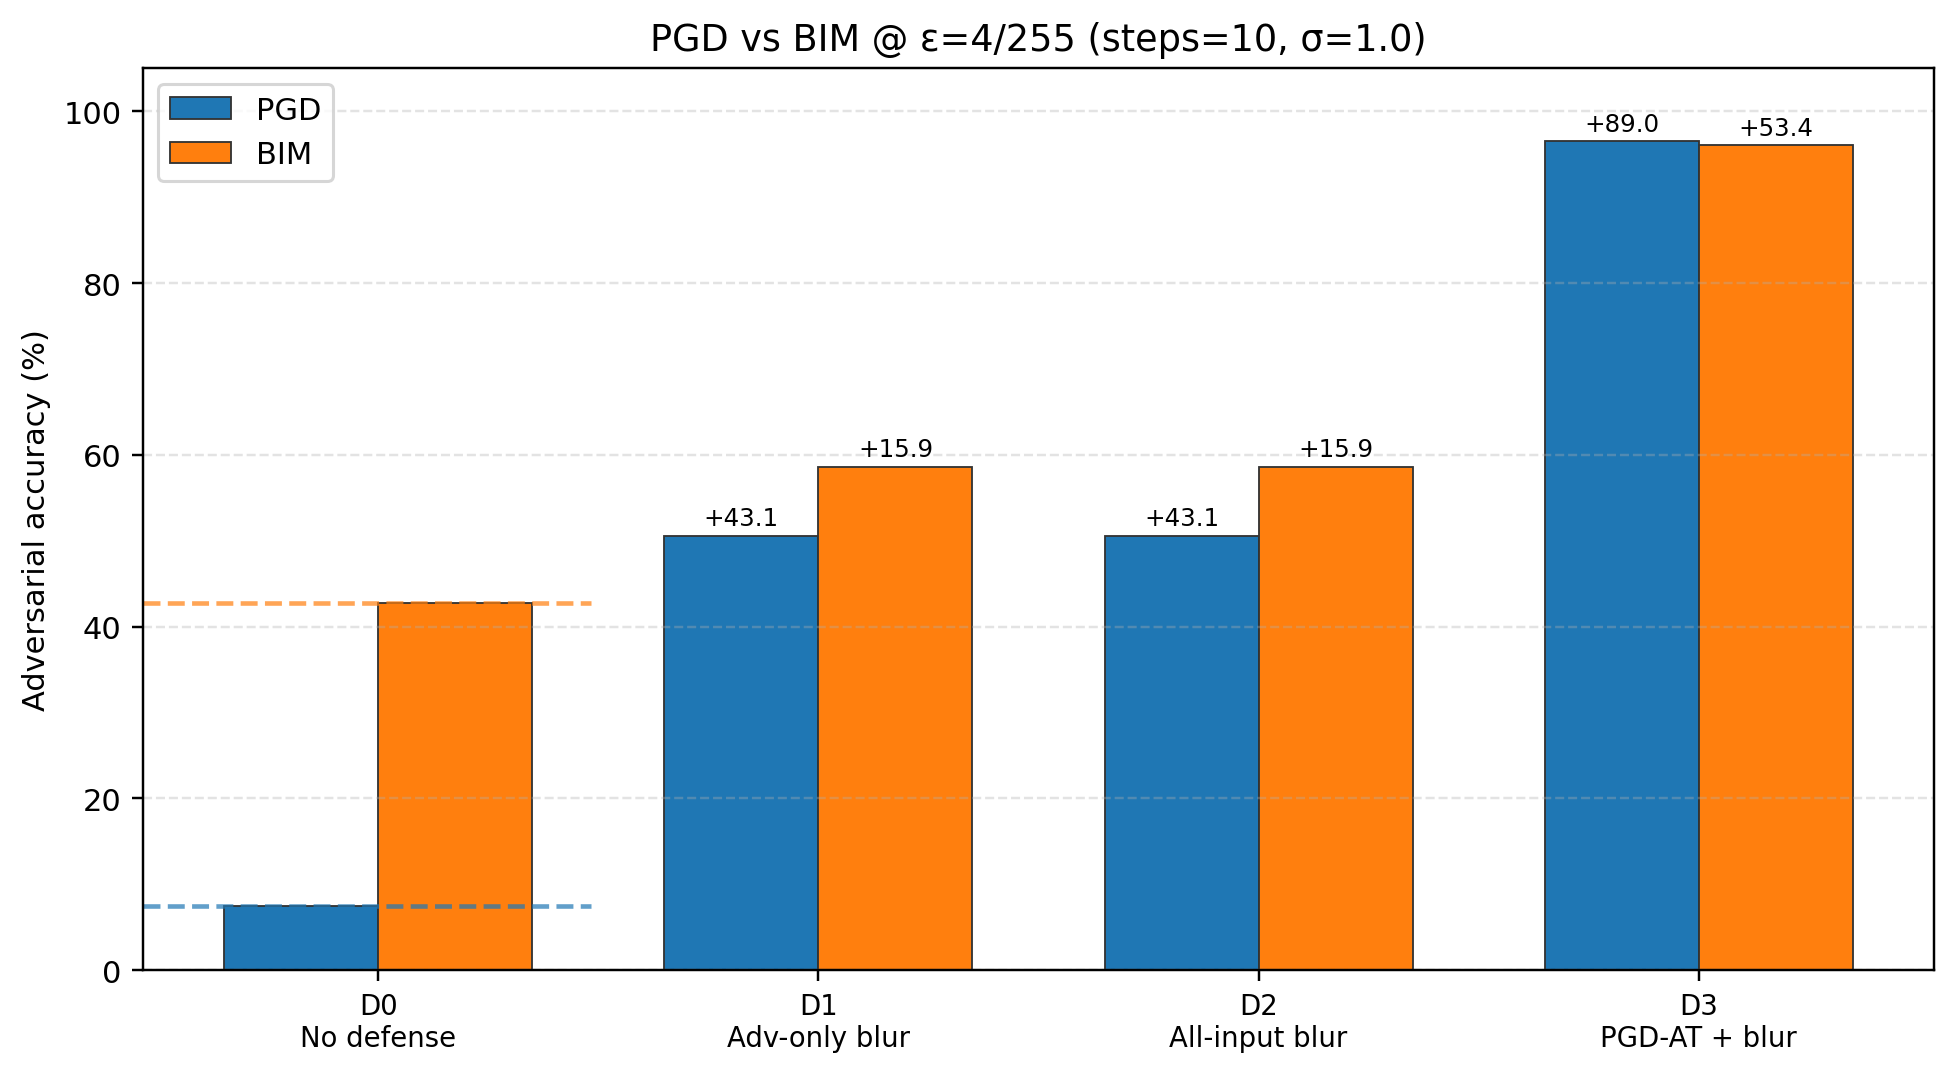
\includegraphics[width=0.82\textwidth]{figures/gaussian_defense_pgd_bim_eps4.png}
  \caption{PGD and BIM robust accuracy at $\epsilon=4/255$ for the four Gaussian smoothing conditions on brain MRI ResNet50.}
  \label{fig:gaussian-factorial}
\end{figure}

Aggregate accuracy does not reveal whether a defence recovers both classes equally. Figure~\ref{fig:gaussian-defence-confusions} shows that undefended PGD at $4/255$ predicts TUMOR for most NO\_TUMOR cases (313 false positives) while predicting NO\_TUMOR for most tumour cases (941 false negatives), indicating widespread boundary crossing in both directions. Gaussian smoothing alone reduces these errors but leaves 149 false positives and 521 false negatives. The combined D3 condition reduces the PGD errors to 33 false positives and 14 false negatives; under BIM it leaves 37 and 16 respectively. The gain is therefore not produced by collapsing to the majority class, but by recovering both class-conditional accuracies.

\begin{figure}[htbp]
  \centering
  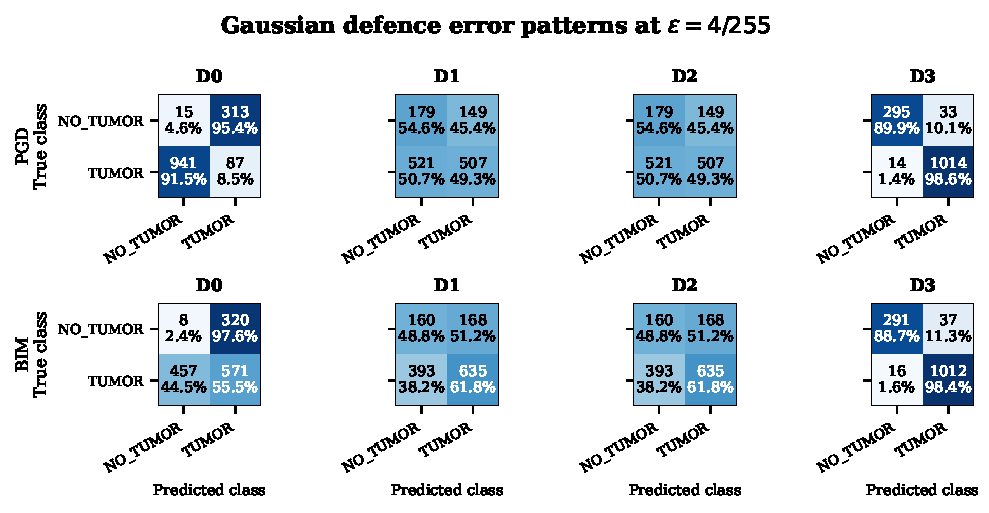
\includegraphics[width=\textwidth]{figures/gaussian_defence_confusion_matrices_eps4.pdf}
  \caption{Confusion matrices for Gaussian defence conditions D0--D3 under PGD and BIM at $\epsilon=4/255$. Cells show counts and within-class percentages.}
  \label{fig:gaussian-defence-confusions}
\end{figure}

\noindent\textit{Key finding.} The defence results show complementary rather than interchangeable effects. Gaussian blur alone recovers part of the lost accuracy, whereas PGD-AT changes the degradation curve across the full range of budgets. Their combination, D3, performs best under both PGD and BIM at $4/255$; however, the sharp decline at $8/255$ confirms that the gain is bounded by the evaluated training budget rather than constituting general protection.

\section{Fair Robustness Summary}
\label{sec:results-fair}

\sectionfocus{Normalising adversarial degradation by each model's clean baseline confirms that the main robustness differences are not merely consequences of unequal clean accuracy.}

Fair robustness normalisation expresses degradation relative to each model's own clean baseline (Section~\ref{sec:methods-metrics}). Under PGD at $\epsilon = 4/255$ on brain MRI, accuracy relative drop was lowest for ResNet50 (92.2\%) and DenseNet121 (96.3\%) among models with non-zero robust accuracy; ConvNeXt-Tiny, ResNet18, and MobileNetV2 reached 100\% relative drop (total collapse). Under FGSM at $\epsilon = 4/255$, ResNet50 showed the lowest accuracy relative drop (45.4\%), followed by DenseNet121 (77.2\%), MobileNetV2 (82.3\%), ResNet18 (84.2\%), and ConvNeXt-Tiny (95.5\%). On chest X-ray under PGD at $\epsilon = 4/255$, ResNet50 accuracy relative drop was 99.8\%, DenseNet121 98.8\%, and ConvNeXt-Tiny and ResNet18 100\%; under FGSM, DenseNet121 showed the lowest relative drop (67.2\%) followed by ConvNeXt-Tiny (75.8\%) and ResNet50 (83.3\%). These normalised metrics confirm that ResNet50 retains the most favourable fair-robustness profile on brain MRI under both FGSM and PGD, while no single architecture dominates fair robustness on chest X-ray across all attacks.

Figure~\ref{fig:fair-retention-heatmaps} extends this comparison to BIM and expresses every cell as the percentage of the corresponding clean accuracy that remains. ResNet50 retains 54.6\% of its brain MRI baseline under FGSM and 43.7\% under BIM, substantially more than the other architectures, but only 14.3\% and 8.5\% on chest X-ray. DenseNet121 retains 28.8\% under chest X-ray FGSM and 26.1\% under BIM, making it the fair-robustness leader for those attacks despite its lower clean accuracy. Under PGD, no chest X-ray model retains even 1.3\% of its baseline at this budget.

\begin{figure}[htbp]
  \centering
  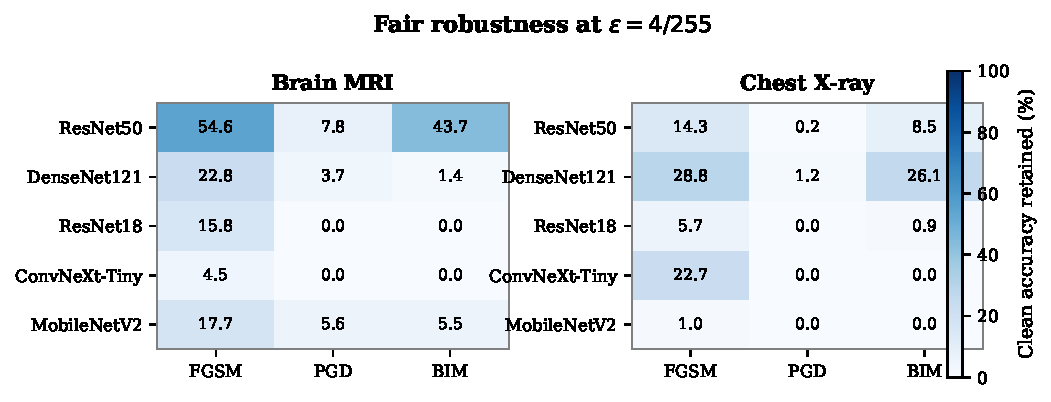
\includegraphics[width=0.94\textwidth]{figures/fair_robustness_retention_eps4.pdf}
  \caption{Clean accuracy retained under FGSM, PGD, and BIM at $\epsilon=4/255$. Normalisation prevents high clean accuracy from being mistaken for robustness.}
  \label{fig:fair-retention-heatmaps}
\end{figure}

\noindent\textit{Key finding.} Normalisation does not overturn the main conclusion: the observed ranking differences are not merely an artefact of unequal clean baselines. ResNet50 remains the least degraded model on brain MRI, while the chest X-ray ranking continues to depend on the selected attack.

\section{Supplementary Attacks: DeepFool and C\&W}
\label{sec:results-supplementary}

\sectionfocus{Alternative attack objectives produce different numerical outcomes and rankings, reinforcing the need to interpret robustness within a clearly specified threat model.}

DeepFool and Carlini--Wagner (C\&W) attacks were evaluated as supplementary benchmarks using formulations distinct from the primary FGSM/PGD/BIM/MIM suite. DeepFool~\cite{moosavi2016deepfool} approximates minimum-norm perturbations with an $L_\infty$ cap after each step; C\&W in this project implements an $L_\infty$-bounded margin attack in logit space (ten steps, $\kappa = 0$). Results in this section are \emph{not} merged into Table~\ref{tab:r50_attack_strength} because the optimisation objectives differ from fixed-budget $L_\infty$ gradient attacks; they are reported separately for completeness.

\subsection{DeepFool}
\label{sec:results-deepfool}

On brain MRI, standard and PGD-AT ResNet50 checkpoints (clean accuracy 97.71\% and 98.82\% respectively) were compared under DeepFool ($L_\infty$ capped, max\_iter=15, overshoot=0.02). Standard ResNet50 robust accuracy was 88.79\%, 74.34\%, 62.76\%, 57.89\%, and 50.07\% at $\epsilon \in \{1,2,3,4,8\}/255$; PGD-AT ResNet50 achieved 98.89\%, 98.60\%, 96.76\%, 93.95\%, and 69.25\% at the same budgets (Table~\ref{tab:deepfool_r50_brain}). Partial five-model DeepFool coverage was obtained on chest X-ray at $\epsilon = 4/255$: DenseNet121 36.30\%, ResNet18 42.81\%, ResNet50 18.38\%, and MobileNetV2 12.56\% robust accuracy, a different architecture ordering from the PGD benchmark at the same $\epsilon$ cap (Table~\ref{tab:deepfool_chest_eps4}). DeepFool robust accuracy values are generally higher than PGD robust accuracy at matched $\epsilon$ caps because DeepFool prioritises smaller perturbations rather than maximising loss within the full $\epsilon$-ball; cross-attack ranking should therefore be interpreted cautiously.

\begin{table}[htbp]
  \centering
  \caption{DeepFool robust accuracy (\%) on brain MRI ResNet50 (standard vs.\ PGD-AT). $L_\infty$ capped; max\_iter=15.}
  \label{tab:deepfool_r50_brain}
  \begin{tabular}{lrrrrr}
    \toprule
    Variant & $\epsilon=1/255$ & $2/255$ & $3/255$ & $4/255$ & $8/255$ \\
    \midrule
    Standard ResNet50 & 88.79 & 74.34 & 62.76 & 57.89 & 50.07 \\
    PGD-AT ResNet50   & 98.89 & 98.60 & 96.76 & 93.95 & 69.25 \\
    \bottomrule
  \end{tabular}
\end{table}

\begin{table}[htbp]
  \centering
  \caption{DeepFool robust accuracy (\%) on chest X-ray at $\epsilon = 4/255$ (partial model coverage).}
  \label{tab:deepfool_chest_eps4}
  \begin{tabular}{lr}
    \toprule
    Model & Robust Acc. (\%) \\
    \midrule
    ResNet18       & 42.81 \\
    DenseNet121    & 36.30 \\
    ResNet50       & 18.38 \\
    MobileNetV2    & 12.56 \\
    \bottomrule
  \end{tabular}
\end{table}

The full DeepFool curves in Figure~\ref{fig:deepfool-defence-curve} show that PGD-AT improves more than the isolated $4/255$ result. The defended model remains above 93\% through $4/255$, while the standard model declines steadily to 57.89\%. At $8/255$, the gap remains 19.18 percentage points, but both curves decline, showing that transfer from PGD training to DeepFool is substantial rather than unlimited.

\begin{figure}[htbp]
  \centering
  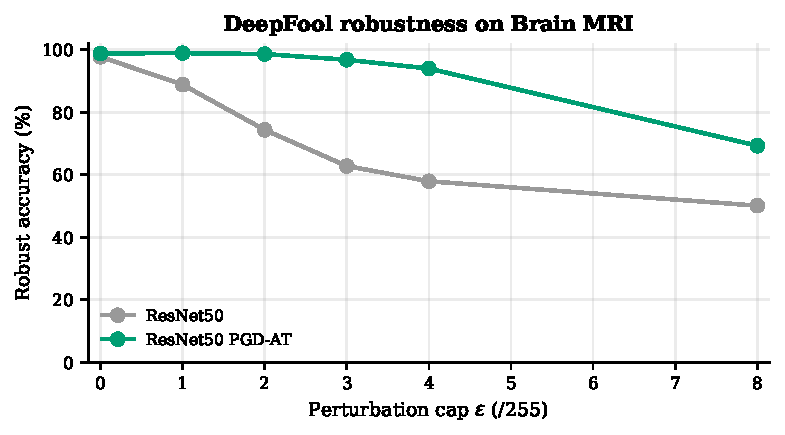
\includegraphics[width=0.78\textwidth]{figures/deepfool_standard_vs_at.pdf}
  \caption{DeepFool robust accuracy across perturbation caps for standard and PGD-adversarially trained ResNet50 on brain MRI.}
  \label{fig:deepfool-defence-curve}
\end{figure}

\noindent\textit{Key finding.} DeepFool produces a different architecture ordering from PGD on chest X-ray, while PGD-AT still improves ResNet50 across all tested caps on brain MRI. This supports the defence result, but not a universal ranking of attack strength, because DeepFool optimises a different objective.

\subsection{Carlini--Wagner ($L_\infty$-bounded)}
\label{sec:results-cw}

C\&W evaluation was completed for ResNet50 only. On chest X-ray (clean accuracy 97.26\%, matching the main protocol), C\&W robust accuracy was 26.83\% at $\epsilon = 2/255$ (ASR 73.17\%) and 26.60\% at $\epsilon = 4/255$ (ASR 73.40\%). A legacy brain MRI C\&W run on an earlier ResNet50 checkpoint (clean accuracy 94.31\%, not the 97.71\% model in Table~\ref{tab:brain_mri_clean_five_models}) reported 17.07\% and 8.94\% robust accuracy at $\epsilon = 2/255$ and $4/255$ respectively (Table~\ref{tab:cw_r50_supplementary}). Chest X-ray C\&W robust accuracy at $\epsilon = 4/255$ (26.60\%) exceeded PGD (0.23\%) and MIM (0.11\%) robust accuracy on the same model and budget, but this comparison mixes attack formulations and should not be read as a strict strength ranking. A full five-model C\&W comparison on the current checkpoints was not conducted owing to computational cost.

\begin{table}[htbp]
  \centering
  \caption{Supplementary C\&W ($L_\infty$-bounded, ten steps) on ResNet50. Brain MRI used an earlier checkpoint (clean 94.31\%); chest X-ray matches the main protocol (clean 97.26\%).}
  \label{tab:cw_r50_supplementary}
  \begin{tabular}{llrrrr}
    \toprule
    Task & Clean Acc. (\%) & $\epsilon$ & Robust Acc. (\%) & ASR (\%) \\
    \midrule
    Brain MRI (legacy) & 94.31 & $2/255$ & 17.07 & 82.93 \\
    Brain MRI (legacy) & 94.31 & $4/255$ &  8.94 & 91.06 \\
    Chest X-ray        & 97.26 & $2/255$ & 26.83 & 73.17 \\
    Chest X-ray        & 97.26 & $4/255$ & 26.60 & 73.40 \\
    \bottomrule
  \end{tabular}
\end{table}

In summary, clean accuracy and adversarial robustness diverged on both tasks: ConvNeXt-Tiny led clean performance but collapsed under iterative $L_\infty$ attacks from $\epsilon = 2/255$; ResNet50 was the most robust standard model on brain MRI but not on chest X-ray; the $L_\infty$ attack-strength ordering on ResNet50 (MIM and PGD strongest, FGSM weakest) was stable across tasks (Table~\ref{tab:r50_attack_strength}); PGD-AT and combined Gaussian smoothing (D3) substantially raised brain MRI robust accuracy at $\epsilon = 4/255$ from 7.52\% to 96.53\% under PGD; DeepFool and C\&W provided supplementary evidence on alternative threat formulations but were not pooled with the primary attack-strength table. Section~5 discusses the implications of these findings for the research objectives stated in Section~1.

\noindent\textit{C\&W caveat.} These results are supplementary evidence rather than a direct cross-task test: the brain MRI checkpoint differs from the main benchmark and only ResNet50 was evaluated. The relatively flat chest X-ray result between $2/255$ and $4/255$ also suggests that this short, bounded optimisation did not exploit the larger budget as strongly as PGD or MIM.

\chapter{Discussion}
\label{ch:discussion}

\sectionfocus{The evidence supports task-specific robustness auditing and layered protection, while cautioning against universal conclusions from a single dataset, attack, or empirical defence.}

Section~4 established that medical image classifiers can achieve high clean accuracy while remaining highly vulnerable to white-box $L_\infty$ adversarial attacks, and that both architecture rankings and absolute robustness levels depend on the clinical task. This section interprets those findings against the research questions posed in Section~1, considers implications for model selection and evaluation in medical AI, examines the defence results on brain MRI, and acknowledges limitations of the experimental design. The discussion follows the structure of the results chapter: within-task behaviour, cross-task transfer, attack-strength stability, defences, and supplementary attacks.

\section{Clean Accuracy and Adversarial Robustness}
\label{sec:disc-clean-robust}

\sectionfocus{The strongest clean classifier is not necessarily the safest choice because standard optimisation and adversarial resilience reward different model behaviour.}

The most consistent finding across both datasets is the decoupling of clean and adversarial performance. Figure~\ref{fig:clean-performance-overview} places the five clean baselines close together at the upper end of the scale, whereas the six panels in Figure~\ref{fig:all-robustness-curves} separate the same models sharply as soon as perturbation is introduced. ConvNeXt-Tiny achieved the highest clean accuracy on brain MRI (98.30\%) and chest X-ray (98.06\%), yet under PGD and BIM it fell to 0\% robust accuracy from $\epsilon = 2/255$ onward on both tasks. The visual contrast is important: the small clean advantage of ConvNeXt-Tiny is overwhelmed by a much larger robustness deficit, so the two evaluation regimes do not merely produce slightly different rankings. This pattern aligns with the robustness--accuracy trade-off discussed by \citet{tsipras2019robustness}: features that minimise standard supervised loss on medical images are not necessarily those that resist gradient-based perturbations. ConvNeXt-Tiny's modern architecture appears well suited to clean generalisation on these binary tasks, but the observed curves are consistent with decision boundaries that iterative attacks can exploit at modest $\epsilon$ budgets. The experiments reveal the behaviour, although they do not isolate which ConvNeXt component causes it.

ResNet50 presents a contrasting profile. It did not lead on clean accuracy on either dataset, but on brain MRI it retained the highest robust accuracy under FGSM, PGD, and BIM at $\epsilon = 4/255$. The brain MRI heatmap in Figure~\ref{fig:robustness-heatmaps} makes this architecture--attack interaction clearer than a single average: ResNet50 retains 53.4\% under FGSM and 42.7\% under BIM, but only 7.6\% under PGD. It is therefore relatively strongest among the evaluated standard models, not robust in an absolute sense. Figure~\ref{fig:fair-retention-heatmaps} reaches the same conclusion after dividing by each model's clean baseline, showing that the result is not an artefact of unequal starting accuracy. The implication for model selection is direct: choosing a classifier by clean validation accuracy alone would favour ConvNeXt-Tiny and potentially deploy one of the least robust options under iterative attacks. Normalisation improves fairness of comparison, but it does not remove the need for explicit adversarial evaluation, because MobileNetV2's lower clean accuracy does not explain its rapid PGD collapse.

On chest X-ray, no single architecture dominated across all attacks after fair normalisation. The right-hand heatmaps in Figures~\ref{fig:robustness-heatmaps} and~\ref{fig:fair-retention-heatmaps} show DenseNet121 preserving more FGSM and BIM performance than ResNet50 despite lower clean accuracy (94.41\% versus 97.26\%), while all five models are nearly eliminated by PGD at $4/255$. This prevents an overly broad interpretation that DenseNet121 is simply ``the robust chest X-ray model'': its advantage depends on the attack, and its PGD retention remains only 1.2\% of clean accuracy. Task-specific decision geometry therefore interacts with architecture in ways that clean benchmarks alone cannot reveal. These observations answer the first research sub-question: within a fixed task and attack protocol, standard fine-tuned models differ substantially in adversarial robustness, and the best clean model is not necessarily the most robust.

The contrast between ConvNeXt-Tiny and ResNet50 deserves explicit emphasis because it encapsulates the robustness--accuracy trade-off in a deployable form. ConvNeXt-Tiny combines the highest clean accuracy on both tasks with the fastest collapse under PGD and BIM from $\epsilon = 2/255$, whereas ResNet50 sacrifices 0.59--0.76 percentage points of clean accuracy relative to ConvNeXt-Tiny yet retains measurable iterative robustness on brain MRI and higher sensitivity retention under PGD at $\epsilon = 2/255$ (70.02\% versus 0\%). A procurement decision based solely on clean validation accuracy would therefore select ConvNeXt-Tiny and accept the weakest iterative-attack profile among the five models evaluated. ResNet50 is not uniformly superior because DenseNet121 outperforms it on chest X-ray under several attacks. Nevertheless, the ConvNeXt-versus-ResNet pairing illustrates why architectural modernity and clean leaderboard rank are insufficient proxies for security-relevant reliability. Prior natural-image work by \citet{tsipras2019robustness} predicted such decoupling in principle; the present dual-dataset results instantiate it in a medical transfer-learning setting with five concurrently trained architectures.

\section{Cross-Task Robustness and Attack-Strength Transfer}
\label{sec:disc-cross-task}

\sectionfocus{Robust model selection must be repeated for the target clinical task, although a common suite of strong iterative attacks remains useful for auditing across modalities.}

Cross-task comparison addressed whether robustness rankings and attack severity generalise between brain MRI and chest X-ray under identical hyperparameters. Figure~\ref{fig:all-robustness-curves} supports a nuanced answer because its left and right columns use identical axes. Architecture rankings are \emph{task-dependent}: the separation of ResNet50 from the other models on brain MRI is not reproduced on chest X-ray, where DenseNet121 often retains the highest FGSM and BIM accuracy. Under PGD at $\epsilon = 4/255$, ResNet50 falls from 7.60\% on brain MRI to 0.23\% on chest X-ray, while DenseNet121 retains 1.14\% on chest X-ray and also leads the other two principal attacks. A hospital or vendor therefore cannot assume that a model validated as relatively robust on one modality will preserve its standing on another, even when the same input resolution and attack implementation are reused.

Absolute robustness was lower on chest X-ray for ResNet50 under every attack in Table~\ref{tab:r50_attack_strength}, suggesting that the pneumonia classification task may present decision boundaries that are easier to fool at fixed $\epsilon$, or that the chest X-ray test distribution interacts differently with $L_\infty$ perturbations. Brain MRI showed higher residual robust accuracy for several models at matched budgets (for example, ResNet50 PGD $\Delta_{\mathrm{robust}} = +7.37$ percentage points at $\epsilon = 4/255$), but the gap narrowed or reversed for other architecture--attack pairs (DenseNet121 FGSM at $\epsilon = 4/255$ was higher on chest X-ray). Cross-task benchmarking is therefore necessary not only for ranking but also for estimating worst-case behaviour in each deployment context.

Attack-strength orderings on the fixed reference model ResNet50 were more stable across tasks. Figure~\ref{fig:r50-attack-strength-bars} shows the same broad pattern in both panels: FGSM leaves the greatest residual accuracy and MIM the least, particularly at $4/255$. The grouped bars also reveal a qualification that a one-budget summary would miss. BIM is more damaging than PGD at $2/255$ but less damaging at $4/255$ on both tasks, so the precise middle ordering changes as the budget increases. The defensible transferable conclusion is therefore not a universal four-attack ranking, but that single-step FGSM is insufficient and that PGD or MIM should be included in auditing. Evaluators can use a common strong attack suite across modalities while still re-running the architecture comparison for each target task.

The supplementary DeepFool and C\&W results caution against over-generalising even this conclusion. DeepFool produced different architecture orderings on chest X-ray at $\epsilon = 4/255$ (ResNet18 highest at 42.81\%, ResNet50 at 18.38\%) because minimum-norm attacks optimise a different objective than fixed-budget PGD. Figure~\ref{fig:deepfool-defence-curve} further shows a gradual DeepFool decline for standard ResNet50 rather than the abrupt PGD collapse in Figure~\ref{fig:all-robustness-curves}. This difference in curve shape is evidence that ``robustness'' is conditional on the attack objective, not a fixed attribute stored in the model. C\&W on chest X-ray ResNet50 likewise yielded higher robust accuracy than PGD at the same cap. Primary conclusions about attack strength therefore rest on the unified $L_\infty$ FGSM/PGD/BIM/MIM protocol; supplementary attacks should be interpreted within their own threat formulations.

\section{Defence Mechanisms and Layered Protection}
\label{sec:disc-defence}

\sectionfocus{Training-time hardening and inference-time filtering are complementary, but their empirical gains remain bounded by perturbation budget and evaluation design.}

Defence experiments on brain MRI evaluated whether training-time adversarial hardening and inference-time Gaussian smoothing could recover usable robustness on the primary task. The standard and defended bars in Figure~\ref{fig:pgd-at-cross-attack} show that PGD-AT does more than memorise the exact training attack: both ResNet50 and DenseNet121 improve under FGSM and BIM as well as PGD. At $\epsilon = 4/255$, PGD robust accuracy rises from 7.60\% to 89.38\% for ResNet50 and from 3.61\% to 88.42\% for DenseNet121. The defended results also cluster within a narrower range across the three attacks, suggesting that PGD-AT reduces attack-specific brittleness in addition to raising average robust accuracy. Figure~\ref{fig:pgd-at-curve} provides the necessary boundary on that interpretation: the advantage persists across the budget sweep but narrows substantially at $8/255$. Min--max training~\cite{madry2018towards} is therefore effective within and near the trained threat region, not evidence of unrestricted robustness. In these runs the defended checkpoints also retained high clean accuracy, so a clean--robust trade-off should not be assumed from theory without measuring it in the specific experiment.

The four-condition Gaussian study (D0--D3) isolated inference-time filtering from training-time hardening. The accuracy bars in Figure~\ref{fig:gaussian-factorial} show partial recovery for D1/D2 and a much larger D3 gain, but Figure~\ref{fig:gaussian-defence-confusions} is more informative about the mechanism's clinical meaning. Under undefended PGD, errors occur heavily in both directions; D3 reduces both false negatives and false positives rather than obtaining high accuracy by predicting the majority TUMOR class. This matters because aggregate recovery could otherwise conceal a clinically unusable operating point. D1 and D2 have identical attacked confusion matrices because both blur adversarial inputs, but only D2 is a deployable non-oracle condition and it lowers clean accuracy to 93.95\%. D3 combines PGD-AT with all-input blur and reaches 96.53\% PGD accuracy while maintaining 98.53\% clean accuracy, supporting complementarity between training-time and inference-time mechanisms. The result remains an empirical benchmark rather than a certification, and the decline at larger budgets prevents the phrase ``clinically usable'' from being inferred from one operating point alone.

Defence results are not extrapolated to chest X-ray in this dissertation. Cross-task attack evaluation showed lower baseline robustness on chest radiographs; whether PGD-AT and Gaussian smoothing would yield similar relative gains is an open question requiring task-specific validation. The brain MRI defence chapter should be read as proof-of-concept on one modality rather than as a universal deployment recipe.

\section{Clinical and Deployment Implications}
\label{sec:disc-clinical}

\sectionfocus{Clinical deployment requires robustness evidence tied to the intended modality, workflow, operating threshold, and computational constraints rather than clean accuracy alone.}

Translating these findings to clinical practice requires separating theoretical adversarial threat from near-term operational risk. White-box $L_\infty$ attacks assume full model access and deliberate perturbation design; such scenarios map most directly to insider threats, compromised PACS workflows, or research red-teaming rather than to every bedside deployment. Nevertheless, \citet{finlayson2019adversarial} showed that medical classifiers can be fooled by small perturbations with diagnostic consequences, and regulators increasingly expect safety evidence beyond clean hold-out performance. This dissertation supports a practical recommendation: any medical imaging product claiming high accuracy should report robustness under at least one iterative attack (PGD or BIM) at clinically motivated $\epsilon$ values, on the target modality, for the deployed architecture.

The asymmetric cost of false negatives versus false positives in pneumonia and tumour screening implies that sensitivity under attack matters alongside accuracy. The clean bars in Figure~\ref{fig:clinical-sensitivity} show sensitivity above 96\% for four architectures on both tasks, making the systems appear similar from a case-detection perspective. The attacked heatmaps beneath them overturn that impression: under PGD at $4/255$, no chest X-ray model retains more than 1.6\% of its clean sensitivity, while brain MRI ResNet50 retains only 8.5\%. In clinical terms, the attack does not merely reduce an abstract score; it largely removes the models' ability to recognise the positive class. The clean confusion matrices in Figure~\ref{fig:clean-confusion-matrices} also show why recall must not be maximised alone. DenseNet121 misses only three chest X-ray pneumonia cases but generates 46 false-positive pneumonia predictions, whereas MobileNetV2 has only three false positives but misses 97 positive cases. A deployment threshold should therefore be selected from an explicit sensitivity--specificity trade-off, and robustness reporting should show how both sides of that trade-off change under attack.

Deployment of layered defences such as condition D3 incurs operational costs that clean-accuracy tables do not capture. PGD-AT requires additional training time proportional to the inner PGD steps per minibatch (ten steps in this project), and all-input Gaussian blur adds a preprocessing pass on every inference request. Neither cost was prohibitive on the RTX~4060 setup used here, and D3 inference remains a single forward pass after blur. However, latency-sensitive emergency radiology workflows would need profiling on hospital hardware before assuming that 96.53\% PGD robust accuracy at $\epsilon = 4/255$ justifies the training and preprocessing overhead. Where retraining is infeasible, condition D1 (blur on adversarial inputs only) is clinically unrealisable because defenders cannot know \emph{a priori} which inputs are adversarial; D2 and D3 apply blur universally and therefore trade a small clean-accuracy reduction for partial robustness without oracle knowledge. These trade-offs suggest that defence selection is a product decision coupling security requirements, compute budget, and acceptable clean-performance regression, not a single universal recommendation.

\section{Limitations}
\label{sec:disc-limitations}

\sectionfocus{The conclusions are empirical rather than universal because attack coverage, defence coverage, datasets, checkpoints, and threat models remain deliberately constrained.}

Several limitations bound the conclusions. The threat model is white-box $L_\infty$ only; black-box, physical-world, and $L_2$ attacks such as Carlini--Wagner in its classical formulation~\cite{carlini2017towards} are not fully characterised. MIM is reported for ResNet50 only; extending attack-strength analysis to all five models would require additional compute. DeepFool coverage is partial, and the brain MRI C\&W evaluation used a legacy checkpoint inconsistent with the main five-model benchmark. PGD-AT and Gaussian experiments are confined to brain MRI; chest X-ray serves as attack-only validation.

All models use ImageNet transfer learning and binary classification at $224 \times 224$ resolution; multi-class tumour subtyping, three-dimensional MRI volumes, and native-resolution radiographs may behave differently. The paediatric chest X-ray dataset and merged brain MRI corpus introduce domain-specific biases. Experiments run on a single GPU with TensorFlow/DirectML; numerical reproducibility is supported by fixed seeds, but PGD random starts introduce residual stochasticity. Finally, robust accuracy above 90\% under D3 at $\epsilon = 4/255$ does not constitute formal certification; randomised smoothing~\cite{cohen2019certified} and other certifiable methods were not evaluated.

Despite these constraints, the dual-dataset, five-architecture design provides a reproducible baseline that addresses gaps identified in Section~2: cross-task comparison, multiple iterative attacks, fair robustness reporting, and factorial defence evaluation on brain MRI. Section~6 summarises how the empirical outcomes map to the stated research objectives, and Section~7 outlines directions for extending the benchmark.

\chapter{Conclusion}
\label{ch:conclusion}

\sectionfocus{Medical image classifiers remain highly vulnerable despite strong clean accuracy, but matched evaluation and combined defences can substantially improve measured resilience.}

This dissertation investigated adversarial robustness in medical image classification across two clinically relevant modalities, brain tumour MRI and paediatric chest X-ray pneumonia detection, using five transfer-learned convolutional architectures, a unified white-box $L_\infty$ attack protocol, cross-task comparison, and layered defence experiments on the primary brain MRI task. The central research question asked how classifiers behave under adversarial attack across medical imaging tasks and to what extent training-time and inference-time defences can mitigate vulnerability. The empirical programme established that clean accuracy and adversarial robustness are largely decoupled, that architecture rankings depend on the clinical task, that attack-strength orderings transfer more reliably than model rankings, and that combined PGD adversarial training with Gaussian smoothing can recover high robust accuracy on brain MRI at moderate perturbation budgets. The following paragraphs summarise how each stated objective was met and what the principal quantitative outcomes imply for the field.

The first objective was to establish a unified dual-dataset benchmark by fine-tuning ResNet50, DenseNet121, ResNet18, MobileNetV2, and ConvNeXt-Tiny under consistent training and evaluation protocols. All five models achieved clean test accuracy above 85\% on both tasks, with ConvNeXt-Tiny leading on brain MRI (98.30\%) and chest X-ray (98.06\%) and ResNet50 achieving 97.71\% and 97.26\% respectively. This objective was fully achieved: the benchmark provides comparable clean baselines, documented training scripts, and LaTeX-ready result tables that can serve as a reference for subsequent medical robustness studies. The benchmark confirms that modern CNNs transfer effectively from ImageNet to binary medical tasks at $224 \times 224$ resolution, but it also reveals that high clean performance does not predict resilience under iterative attacks.

The second objective was to characterise within-task adversarial robustness using FGSM, PGD, and BIM across $\epsilon \in \{1,2,3,4,8\}/255$. On brain MRI at $\epsilon = 4/255$, PGD reduced ConvNeXt-Tiny and ResNet18 to 0\% robust accuracy, while DenseNet121 retained 3.61\%, MobileNetV2 4.79\%, and ResNet50 7.60\%. Under BIM at the same budget, ResNet50 again led with 42.70\%, followed by MobileNetV2 at 4.72\%, DenseNet121 at 1.33\%, and total collapse for ResNet18 and ConvNeXt-Tiny. Fair robustness normalisation, which scales each model's robust accuracy by its clean baseline, confirmed ResNet50 as the least degraded standard model under FGSM, PGD, and BIM on brain MRI. On chest X-ray, the pattern diverged: DenseNet121 showed higher FGSM and BIM robustness at $\epsilon = 4/255$ than ResNet50 despite lower clean accuracy, and no single architecture dominated all attack types after fair normalisation. The objective was met with the qualification that robustness rankings are task-specific; evaluators cannot select a universally ``most robust'' architecture from these two datasets alone.

The third objective was to compare cross-task robustness and attack-strength profiles at matched perturbation budgets. ResNet50 PGD robust accuracy fell from 7.60\% on brain MRI to 0.23\% on chest X-ray at $\epsilon = 4/255$, demonstrating that a model's relative and absolute robustness on one modality does not transfer to another under identical attack code. Architecture rankings reversed or narrowed for several attack--model pairs: DenseNet121 outperformed ResNet50 on chest X-ray under FGSM and BIM at $\epsilon = 4/255$, whereas ResNet50 led on brain MRI under PGD. In contrast, attack-strength ordering on the fixed reference model ResNet50 was stable: at $\epsilon = 4/255$, both tasks ranked FGSM as the weakest attack and MIM as the strongest, with PGD consistently more damaging than BIM on brain MRI. Cross-task benchmarking is therefore necessary for model selection per deployment context, while a common strong attack suite (PGD or MIM rather than FGSM alone) can be adopted across modalities for threat modelling. Supplementary DeepFool and Carlini--Wagner evaluations on chest X-ray further showed that minimum-norm and margin-based attacks can reorder architecture rankings relative to fixed-budget PGD, reinforcing the need to align evaluation with the intended threat model.

The fourth objective was to evaluate PGD adversarial training and Gaussian smoothing on brain MRI, individually and in combination. PGD-AT raised ResNet50 PGD robust accuracy at $\epsilon = 4/255$ from 7.60\% to 89.38\% and DenseNet121 from 3.61\% to 88.42\%, with cross-attack transfer to BIM and FGSM. The four-condition Gaussian protocol showed that inference-time blur on adversarial inputs alone (D1) or on all inputs (D2) improved PGD robust accuracy at $\epsilon = 4/255$ from 7.52\% (D0) to approximately 50.59\% without retraining, at a modest clean-accuracy cost when blur was applied universally. Condition D3, combining PGD-AT with all-input Gaussian smoothing, achieved 96.53\% PGD robust accuracy at $\epsilon = 4/255$ while maintaining 98.53\% clean accuracy, a substantial improvement over either mechanism alone. These results demonstrate that layered defences can approach clinically usable robustness levels on this benchmark at moderate $\epsilon$, though robustness at $\epsilon = 8/255$ remains limited even under D3. Defence experiments were intentionally confined to brain MRI; chest X-ray served as attack-only validation, and extrapolating defence gains to chest radiographs would require task-specific replication.

Taken together, the dissertation answers the central research question as follows. Convolutional classifiers trained for medical binary classification exhibit substantial and architecture-dependent vulnerability to white-box $L_\infty$ attacks; the best clean model (ConvNeXt-Tiny) was among the least robust under iterative attacks on both tasks. Robustness rankings and absolute robust accuracy levels differ between brain MRI and chest X-ray, so cross-task evaluation is essential before deployment in multi-modality settings. Attack-strength orderings on a reference model transfer more reliably than model rankings, supporting standardised strong attacks for comparative auditing. On brain MRI, PGD-AT and Gaussian smoothing individually improve robustness, and their combination (D3) yields the strongest empirical protection within the evaluated protocol. The work does not claim formal robustness certification or universal clinical readiness; rather, it provides a reproducible evidence base that complements clean benchmark reporting with adversarial metrics, fair normalisation, and cross-task framing, addressing gaps identified in the related-work review.

The contributions of this dissertation are empirical and methodological rather than theoretical. It delivers a dual-dataset, five-architecture robustness benchmark under unified hyperparameters; a systematic cross-task analysis distinguishing task-dependent model behaviour from more stable attack orderings; an factorial defence evaluation on brain MRI isolating training-time hardening, inference-time filtering, and their combination; and transparent reporting artefacts including comparison tables and documented experimental pipelines. For practitioners, the principal takeaway is procedural: report robust accuracy under at least one iterative attack on the target modality and architecture before claiming reliability; do not assume that clean leaderboard performance or robustness on one dataset generalises to another; and consider layered defences where compute and latency constraints permit. For researchers, the benchmark establishes a baseline against which additional modalities, attacks, and certified methods can be compared under the same reproducible framework outlined in Section~3.

In closing, medical AI systems that achieve high accuracy on retrospective clean data remain vulnerable to adversarial perturbations at budgets small relative to pixel dynamic range. This vulnerability is not uniform across architectures or clinical tasks, and it can be partially mitigated on brain MRI through adversarial training and input smoothing used together. The dissertation fulfils its stated objectives within the defined white-box $L_\infty$ scope and contributes evidence that cross-task robustness evaluation should be treated as a first-class requirement in medical machine learning safety research, not an optional extension to single-dataset studies. Section~7 identifies concrete directions for extending this work beyond the boundaries of the present experiments.

\section{Answers to the Research Questions}

\paragraph{RQ1: How does model architecture influence adversarial robustness?}
The difference is substantial and is not explained by clean accuracy. On brain MRI at $\epsilon=4/255$, ResNet50 retained 7.60\% accuracy under PGD, while ResNet18 and ConvNeXt-Tiny reached 0\%; under FGSM, the range extended from 53.39\% for ResNet50 to 4.42\% for ConvNeXt-Tiny. ConvNeXt-Tiny nevertheless achieved the highest clean accuracy on both datasets. The answer to RQ1 is therefore that architectures with similar clean performance can have markedly different adversarial behaviour, and clean accuracy is not a reliable proxy for robustness.

\paragraph{RQ2: Does adversarial robustness vary across tasks and datasets?}
Adversarial robustness varied substantially between the two classification settings, both in absolute accuracy and in the relative ranking of architectures.
No consistent architecture ranking transferred from brain MRI to chest X-ray. ResNet50 was the strongest standard model on brain MRI under the principal attacks, whereas DenseNet121 achieved the highest chest X-ray robustness under FGSM, PGD, and BIM at the reported $2/255$ and $4/255$ budgets. ResNet50 PGD accuracy also fell from 7.60\% on brain MRI to 0.23\% on chest X-ray at $4/255$. The answer to RQ2 is therefore that robustness is strongly task- and dataset-dependent and must be measured in the intended deployment domain.

\paragraph{RQ3: Is the relative effectiveness of adversarial attacks stable across tasks?}
It is more stable than the architecture ranking, although not identical at every budget. For ResNet50 at $4/255$, both datasets placed FGSM as the weakest and MIM as the strongest attack; PGD and BIM lay between them. At $2/255$, the relative position of PGD and BIM varied, but MIM still produced the highest attack success rate. Thus, the broad conclusion transfers across tasks: single-step FGSM is insufficient as the sole robustness test, and a strong iterative attack should be included. Fine-grained rankings, however, remain budget-dependent.

\paragraph{RQ4: How much can training-time and inference-time defences improve robustness?}
Both improved brain MRI robustness, but their combination was strongest. At $4/255$, PGD-AT increased ResNet50 PGD accuracy from 7.60\% to 89.38\%. Gaussian blur without adversarial training increased the corresponding D0 result from 7.52\% to 50.59\%, while D3 (PGD-AT plus all-input blur) reached 96.53\% under PGD and 96.09\% under BIM. RQ4 is therefore answered within the evaluated threat model: training-time hardening and inference-time smoothing are complementary, although the decline at $8/255$ and the absence of formal certification prevent a claim of general or clinical robustness.

\chapter{Future Work}
\label{ch:future}

\sectionfocus{The most important extensions are broader attack coverage, cross-task defence replication, certified guarantees, stronger statistical reporting, and clinically grounded evaluation.}

The experiments reported in this dissertation establish a reproducible dual-dataset benchmark and several actionable findings, but they also expose limitations that define a natural research agenda. Future work can extend along four axes: broadening the threat model and attack coverage; expanding datasets, modalities, and task complexity; deepening and generalising defence evaluation; and strengthening the link between empirical robustness and clinical deployment requirements including certification, latency, and regulatory evidence. Each axis below builds directly on gaps acknowledged in Sections~5 and~6 and on the experimental infrastructure already documented in the project repository.

A first priority is to complete and harmonise attack coverage across all five architectures. MIM was evaluated only on ResNet50 for attack-strength comparison; extending MIM, and potentially other momentum-based or adaptive attacks, to DenseNet121, ResNet18, MobileNetV2, and ConvNeXt-Tiny would test whether the FGSM~$<$~BIM~$<$~PGD~$<$~MIM ordering observed on ResNet50 holds architecture-wide or is itself model-dependent. DeepFool coverage remains partial: brain MRI results exist for some models but not the full five-model matrix, and chest X-ray DeepFool at $\epsilon = 4/255$ produced different architecture rankings than PGD because minimum-norm attacks optimise a different objective. A systematic DeepFool sweep with consistent checkpoint selection would clarify whether ResNet18's relative strength under DeepFool on chest X-ray reflects genuine boundary geometry or experimental artefacts. The Carlini--Wagner evaluation on chest X-ray used a legacy ResNet50 checkpoint inconsistent with the main benchmark; re-running C\&W with the unified five-model checkpoints would allow fair comparison between $L_2$ margin-based and $L_\infty$ loss-maximisation attacks. Black-box and grey-box threat models were outside scope but are highly relevant to deployment scenarios where model weights are not exposed to end users. Examples include query-limited score-based attacks, transfer attacks from surrogate models, and physically realisable perturbations applied to displayed radiographs.

Cross-task defence generalisation represents a second major extension. PGD-AT and the Gaussian D0--D3 protocol were applied only to brain MRI; chest X-ray showed lower baseline robustness for several models under matched attacks, and it is unknown whether adversarial training would yield proportional gains (for example, raising ResNet50 from 0.23\% to a usable robust accuracy band at $\epsilon = 4/255$) or whether the pneumonia task's decision boundaries respond differently to min--max training. Replicating the PGD-AT and factorial Gaussian design on chest X-ray, and optionally training a single multi-task model on both datasets, would test whether defence recipes transfer across modalities or require task-specific tuning. Multi-class brain tumour subtyping (glioma, meningioma, pituitary, and related labels present in the source corpus before binary merging) would increase decision-boundary complexity and may reduce the extreme collapse observed under PGD for several architectures; evaluating robustness in multi-class settings aligns better with clinical reporting requirements than binary NO\_TUMOR versus TUMOR alone.

Third, architectural and representational extensions would stress-test the clean-versus-robust decoupling observed for ConvNeXt-Tiny. Vision transformers and hybrid architectures (ConvNeXt at larger scales, Swin Transformer, ViT with medical pretraining) are increasingly deployed in research pipelines; including them in the same attack protocol would reveal whether the robustness--accuracy trade-off documented for CNNs extends to attention-based models. Three-dimensional volumetric MRI classification, which preserves spatial context lost when individual slices are resized to $224 \times 224$, may exhibit different adversarial sensitivity because perturbations can be distributed across depth; adapting the benchmark to 3D ResNet or nnU-Net-style encoders would bridge the gap between slice-based academic experiments and clinical PACS workflows. Native-resolution evaluation (512~px or full DICOM dimensions) would test whether downsampling to ImageNet-compatible inputs artificially inflates or deflates perceived robustness by smoothing high-frequency attack components.

Certified and theoretically grounded defences form a fourth extension axis. Randomised smoothing~\cite{cohen2019certified} provides provable $L_2$ robustness guarantees at the cost of multiple forward passes and calibrated noise levels; implementing certified evaluation on the brain MRI and chest X-ray benchmarks would complement the empirical PGD robust accuracy reported here and support claims that exceed ``best effort'' adversarial training. Interval bound propagation, Lipschitz-constrained training, and TRADES-style regularisation represent alternative training objectives that may achieve better clean--robust Pareto fronts than standard PGD-AT alone. Comparing D3 (PGD-AT plus Gaussian blur) against certified smoothing at matched compute budgets would inform whether inference-time filtering remains competitive when formal guarantees are required. Ensemble adversarial training~\cite{tramer2018ensemble} and feature denoising~\cite{xie2019feature} cited in Section~2 were not implemented; they could be added as additional rows in the defence comparison without changing the core benchmark structure.

Clinical and operational follow-up should connect robustness metrics to workflow constraints. Hospital deployment imposes latency ceilings, GPU availability, and audit requirements that the present offline TensorFlow experiments do not model. Measuring throughput and memory for D3 inference (PGD-AT model plus Gaussian preprocessing) relative to the standard model would quantify the operational cost of layered defence. Prospective evaluation with radiologist-in-the-loop review of adversarially perturbed images, including perceptual studies asking whether PGD perturbations at $\epsilon = 4/255$ are visually detectable on medical displays, would ground the white-box threat model in human factors. Regulatory frameworks increasingly reference robustness and safety; packaging the benchmark scripts, seeds, and result tables as an open reproducibility bundle would allow independent verification and could support future conformity assessment documentation, though formal regulatory submission lies beyond a dissertation scope.

Finally, methodological refinements would strengthen cross-study comparability. Reporting confidence intervals via bootstrap resampling over the test set, or fixed multiple random PGD initialisations with variance bands, would characterise stochastic attack variability omitted from single-run tables. Extending fair robustness metrics to include sensitivity, specificity, and area under the ROC curve under attack would better reflect asymmetric clinical costs discussed in Section~1. Federated or multi-site robustness evaluation, where models trained on one hospital's data are attacked on another site's distribution shift, would test whether adversarial vulnerability compounds with domain shift, a realistic concern for deployed medical AI.

In summary, the present dissertation provides a foundation for dual-dataset, multi-architecture adversarial evaluation in medical imaging; the most impactful near-term extensions are cross-task defence replication on chest X-ray, complete MIM and DeepFool coverage across all models, certified robustness baselines, and black-box threat models aligned with deployment assumptions. Longer-term work should integrate volumetric imaging, native-resolution pipelines, and clinician-centred validation so that robustness research keeps pace with the modalities and governance expectations of real clinical AI systems.

% =============================================================================
% References
% =============================================================================
\bibliographystyle{plainnat}
\begin{thebibliography}{99}

\bibitem[Carlini and Wagner(2017)]{carlini2017towards}
Carlini, N. and Wagner, D. (2017).
\newblock Towards evaluating the robustness of neural networks.
\newblock In \emph{Proceedings of the IEEE Symposium on Security and Privacy (S\&P)}, pages 39--57.

\bibitem[Cohen et~al.(2019)]{cohen2019certified}
Cohen, J., Rosenfeld, E., and Kolter, Z. (2019).
\newblock Certified adversarial robustness via randomized smoothing.
\newblock In \emph{Proceedings of the 36th International Conference on Machine Learning (ICML)}, pages 1310--1320.

\bibitem[Deng et~al.(2009)]{deng2009imagenet}
Deng, J., Dong, W., Socher, R., Li, L.-J., Li, K., and Fei-Fei, L. (2009).
\newblock ImageNet: A large-scale hierarchical image database.
\newblock In \emph{Proceedings of the IEEE Conference on Computer Vision and Pattern Recognition (CVPR)}, pages 248--255.

\bibitem[Dong et~al.(2018)]{dong2018mim}
Dong, Y., Liao, F., Pang, T., Su, H., Zhu, J., Hu, X., and Li, J. (2018).
\newblock Boosting adversarial attacks with momentum.
\newblock In \emph{Proceedings of the IEEE Conference on Computer Vision and Pattern Recognition (CVPR)}, pages 9185--9193.

\bibitem[Dong et~al.(2023)]{dong2023survey}
Dong, J., Chen, J., Xie, X., Lai, J., and Chen, H. (2023).
\newblock Survey on adversarial attack and defense for medical image analysis: Methods and challenges.
\newblock \emph{arXiv preprint arXiv:2303.14133}.

\bibitem[Esteva et~al.(2017)]{esteva2017dermatologist}
Esteva, A., Kuprel, B., Novoa, R. A., Ko, J., Swetter, S. M., Blau, H. M., and Thrun, S. (2017).
\newblock Dermatologist-level classification of skin cancer with deep neural networks.
\newblock \emph{Nature}, 542(7639):115--118.

\bibitem[Finlayson et~al.(2019)]{finlayson2019adversarial}
Finlayson, S. G., Bowers, J. D., Ito, J., Li, N. L., and Beam, A. L. (2019).
\newblock Adversarial attacks on medical machine learning.
\newblock \emph{Science}, 363(6433):1287--1289.

\bibitem[Goodfellow et~al.(2015)]{goodfellow2015explaining}
Goodfellow, I. J., Shlens, J., and Szegedy, C. (2015).
\newblock Explaining and harnessing adversarial examples.
\newblock In \emph{Proceedings of the International Conference on Learning Representations (ICLR)}.

\bibitem[Ghamizi et~al.(2023)]{ghamizi2023evaluating}
Ghamizi, S., Cordy, M., Papadakis, M., and Le Traon, Y. (2023).
\newblock On evaluating adversarial robustness of chest X-ray classification: Pitfalls and best practices.
\newblock In \emph{AAAI Workshop on Artificial Intelligence Safety (SafeAI)}.

\bibitem[Guo et~al.(2020)]{guo2020mechanism}
Guo, C., Rana, M., C{\u{a}}linescu, R., and Ko, C. (2020).
\newblock Spatio-temporal patterns as a deep learning defence against adversarial attacks.
\newblock \emph{arXiv preprint arXiv:2002.08306}.

\bibitem[He et~al.(2016)]{he2016deep}
He, K., Zhang, X., Ren, S., and Sun, J. (2016).
\newblock Deep residual learning for image recognition.
\newblock In \emph{Proceedings of the IEEE Conference on Computer Vision and Pattern Recognition (CVPR)}, pages 770--778.

\bibitem[Huang et~al.(2017)]{huang2017densely}
Huang, G., Liu, Z., Van Der Maaten, L., and Weinberger, K. Q. (2017).
\newblock Densely connected convolutional networks.
\newblock In \emph{Proceedings of the IEEE Conference on Computer Vision and Pattern Recognition (CVPR)}, pages 4700--4708.

\bibitem[Hirano et~al.(2021)]{hirano2021universal}
Hirano, H., Minagi, A., and Takemoto, K. (2021).
\newblock Universal adversarial attacks on deep neural networks for medical image classification.
\newblock \emph{BMC Medical Imaging}, 21.
\newblock doi:10.1186/s12880-020-00530-y.

\bibitem[Kermany et~al.(2018)]{kermany2018identifying}
Kermany, D. S., Goldbaum, M., Cai, W., Valentim, C. C., Liang, H., Baxter, S. L., et~al. (2018).
\newblock Identifying medical diagnoses and treatable diseases by image-based deep learning.
\newblock \emph{Cell}, 172(5):1122--1131.

\bibitem[Kurakin et~al.(2017)]{kurakin2017adversarial}
Kurakin, A., Goodfellow, I., and Bengio, S. (2017).
\newblock Adversarial machine learning at scale.
\newblock In \emph{Proceedings of the International Conference on Learning Representations (ICLR)}.

\bibitem[Litjens et~al.(2017)]{litjens2017survey}
Litjens, G., Kooi, T., Bejnordi, B. E., Setio, A. A. A., Ciompi, F., Ghafoorian, M., et~al. (2017).
\newblock A survey on deep learning in medical image analysis.
\newblock \emph{Medical Image Analysis}, 42:60--88.

\bibitem[Li et~al.(2020)]{li2020defending}
Li, X., Pan, D., and Zhu, D. (2020).
\newblock Defending against adversarial attacks on medical imaging AI system, classification or detection?
\newblock \emph{arXiv preprint arXiv:2006.13555}.

\bibitem[Liu et~al.(2022)]{liu2022convnet}
Liu, Z., Mao, H., Wu, C.-Y., Feichtenhofer, C., Darrell, T., and Xie, S. (2022).
\newblock A ConvNet for the 2020s.
\newblock In \emph{Proceedings of the IEEE/CVF Conference on Computer Vision and Pattern Recognition (CVPR)}, pages 11976--11986.

\bibitem[Ma et~al.(2021)]{ma2021understanding}
Ma, X., Niu, Y., Gu, L., Wang, Y., Zhao, Y., Bailey, J., and Lu, F. (2021).
\newblock Understanding adversarial attacks on deep learning based medical image analysis systems.
\newblock \emph{Pattern Recognition}, 110:107332.

\bibitem[Madry et~al.(2018)]{madry2018towards}
Madry, A., Makelov, A., Schmidt, L., Tsipras, D., and Vladu, A. (2018).
\newblock Towards deep learning models resistant to adversarial attacks.
\newblock In \emph{Proceedings of the International Conference on Learning Representations (ICLR)}.

\bibitem[Moosavi-Dezfooli et~al.(2016)]{moosavi2016deepfool}
Moosavi-Dezfooli, S.-M., Fawzi, A., and Frossard, P. (2016).
\newblock DeepFool: A simple and accurate method to fool deep neural networks.
\newblock In \emph{Proceedings of the IEEE Conference on Computer Vision and Pattern Recognition (CVPR)}, pages 2574--2582.

\bibitem[Paschali et~al.(2018)]{paschali2018generalizability}
Paschali, M., Conjeti, S., Navarro, F., and Navab, N. (2018).
\newblock Generalizability vs.\ robustness: Adversarial examples for medical imaging.
\newblock In \emph{Medical Image Computing and Computer Assisted Intervention (MICCAI)}.

\bibitem[Papernot et~al.(2017)]{papernot2017practical}
Papernot, N., McDaniel, P., Goodfellow, I., Jha, S., Celik, Z. B., and Swami, A. (2017).
\newblock Practical black-box attacks against machine learning.
\newblock In \emph{Proceedings of the 2017 ACM on Asia Conference on Computer and Communications Security (AsiaCCS)}, pages 506--519.

\bibitem[Rajpurkar et~al.(2017)]{rajpurkar2017chexnet}
Rajpurkar, P., Irvin, J., Zhu, K., Yang, B., Mehta, H., Duan, T., et~al. (2017).
\newblock CheXNet: Radiologist-level pneumonia detection on chest X-rays with deep learning.
\newblock \emph{arXiv preprint arXiv:1711.05225}.

\bibitem[Rodriguez et~al.(2022)]{rodriguez2022complexity}
Rodriguez, D., Nayak, T., Krishnan, R., Huang, Y., and Chen, Y. (2022).
\newblock On the role of deep learning model complexity in adversarial robustness for medical images.
\newblock \emph{BMC Medical Informatics and Decision Making}, 22.
\newblock doi:10.1186/s12911-022-01891-w.

\bibitem[Sandler et~al.(2018)]{sandler2018mobilenetv2}
Sandler, M., Howard, A., Zhu, M., Zhmoginov, A., and Chen, L.-C. (2018).
\newblock MobileNetV2: Inverted residuals and linear bottlenecks.
\newblock In \emph{Proceedings of the IEEE Conference on Computer Vision and Pattern Recognition (CVPR)}, pages 4510--4520.

\bibitem[Szegedy et~al.(2014)]{szegedy2014intriguing}
Szegedy, C., Zaremba, W., Sutskever, I., Bruna, J., Erhan, D., Goodfellow, I., and Fergus, R. (2014).
\newblock Intriguing properties of neural networks.
\newblock In \emph{Proceedings of the International Conference on Learning Representations (ICLR)}.

\bibitem[Tramer et~al.(2018)]{tramer2018ensemble}
Tramer, F., Kurakin, A., Papernot, N., Goodfellow, I., Boneh, D., and McDaniel, P. (2018).
\newblock Ensemble adversarial training: Attacks and defenses.
\newblock In \emph{Proceedings of the International Conference on Learning Representations (ICLR)}.

\bibitem[Tsipras et~al.(2019)]{tsipras2019robustness}
Tsipras, D., Santurkar, S., Engstrom, L., Turner, A., and Madry, A. (2019).
\newblock Robustness may be at odds with accuracy.
\newblock In \emph{Proceedings of the International Conference on Learning Representations (ICLR)}.

\bibitem[Xie et~al.(2019)]{xie2019feature}
Xie, C., Tan, M., Gong, B., Yuille, A., and Le, Q. V. (2019).
\newblock Adversarial examples improve image recognition.
\newblock In \emph{Proceedings of the IEEE/CVF Conference on Computer Vision and Pattern Recognition (CVPR)}, pages 819--828.

\end{thebibliography}

\end{document}


